\documentclass[11pt]{article}

\usepackage[margin=1in]{geometry}
\usepackage[T1]{fontenc}
\usepackage[utf8]{inputenc}
\usepackage{lmodern}
\usepackage{microtype}
\usepackage{graphicx}
\usepackage{booktabs}
\usepackage{longtable}
\usepackage{tabularx}
\usepackage{array}
\usepackage{multirow}
\usepackage{pdflscape}
\usepackage{hyperref}
\usepackage{xurl}
\usepackage{float}
\usepackage{caption}
\usepackage{subcaption}
\usepackage{enumitem}
\usepackage{amsmath,amssymb}
\usepackage{xcolor}
\usepackage{colortbl}
\usepackage{fancyhdr}
\usepackage{setspace}

% Colors for official vs local distinction
\definecolor{officialblue}{HTML}{1F4E79}
\definecolor{localgreen}{HTML}{2E7D32}
\definecolor{officialbg}{HTML}{E8F0FE}
\definecolor{localbg}{HTML}{E8F5E9}
\definecolor{gapred}{HTML}{C62828}

\hypersetup{
  colorlinks=true,
  linkcolor=blue!70!black,
  urlcolor=blue!80!black,
  citecolor=green!50!black
}

\setlist[itemize]{leftmargin=*, topsep=4pt, itemsep=2pt}
\setlist[enumerate]{leftmargin=*, topsep=4pt, itemsep=2pt}

\graphicspath{{figures/}}

\pagestyle{fancy}
\fancyhf{}
\fancyhead[L]{\small Reproducibility Study: WavesFM}
\fancyhead[R]{\small\thepage}
\renewcommand{\headrulewidth}{0.4pt}

\setstretch{1.15}

\newcommand{\code}[1]{\texttt{#1}}

\title{
    \textbf{Reproducibility Study of WavesFM:\\A Multimodal Wireless Foundation Model}\\[0.4cm]
    \large Local Benchmarks, Dataset Audits, and Cross-System Execution
}
\author{
    Maheen Fatima\\
    \textit{Department of Electrical and Software Engineering}\\
    \textit{University of Calgary, Canada}
}
\date{April 2026}

\begin{document}

\maketitle

% ============================================================
\begin{abstract}
This report documents a reproducibility study of WavesFM, a multimodal wireless foundation model that uses a shared Vision Transformer backbone to process both raw IQ signals and image-like wireless data across multiple downstream tasks. Starting from the publicly released code, pretrained checkpoint, and dataset instructions, every preprocessing cache was rebuilt, the code was adapted for the available hardware, and the complete benchmark suite---a total of 126 individual training runs across three experimental sessions---was executed on a university lab GPU server. The results are encouraging but mixed. Eight of the ten attempted tasks reproduced closely: RF fingerprinting, modulation classification, 5G NR positioning, UWB indoor and industrial localization, RADCOM signal classification, interference classification, and DeepMIMO LoS/NLoS all fell within a fraction of a percentage point of the published numbers. Human activity sensing also came close, though with a caveat about the data splitting protocol. DeepMIMO beam prediction, however, showed a persistent 9--11 percentage point gap that survived three corrective attempts, pointing to an underspecified benchmark artifact that is not publicly available. One additional task, RF signal classification, could not be attempted because the publicly available raw data does not match the format the code expects.
\end{abstract}

\newpage
\tableofcontents
\newpage

% ============================================================
%  1  Introduction
% ============================================================
\section{Introduction}
\label{sec:intro}

\subsection{The Problem: Too Many Models, Not Enough Reuse}

Modern wireless communication systems---the networks behind WiFi, 5G, Bluetooth, and emerging 6G---generate data at every stage of the signal processing chain. When a phone connects to a cell tower, the radio signals can be captured as raw waveforms, processed into frequency-domain representations called \textit{spectrograms}, analyzed as \textit{channel state information} (CSI) that describes how the signal traveled through the environment, or examined as \textit{channel impulse responses} (CIR) that show how the signal bounced off surfaces over time.

Each of these data types is useful for different tasks. CSI can reveal what activity a person is performing in a room (sensing). Spectrograms can identify what kind of radio signal is being transmitted (classification). Raw waveforms can fingerprint which specific device sent a signal (identification). Channel data can estimate where a user is located (positioning).

Traditionally, each of these tasks requires its own specially designed machine learning model, its own training pipeline, and its own dataset. Building a WiFi sensing model teaches the system nothing about 5G positioning. A modulation classifier shares no knowledge with an interference detector. This fragmented approach is expensive: every new task starts from scratch.

\subsection{The Foundation Model Approach}

In other areas of artificial intelligence, a different paradigm has gained traction: \textit{foundation models}. Instead of training a separate model for each task, a single model is trained on a broad variety of unlabeled data. This pretrained model learns general-purpose features---patterns and structures that are useful across many different tasks. For any specific task, the pretrained model is then adapted with a smaller amount of task-specific training, a process called \textit{fine-tuning}. This is the approach behind well-known models like GPT (for language) and CLIP (for images).

WavesFM asks whether this same approach can work for wireless signals.

\subsection{What WavesFM Is}

WavesFM~\cite{wavesfm_paper,wavesfm_original} is a multimodal wireless foundation model developed by Ahmed Aboulfotouh and Hatem Abou-Zeid at the University of Calgary. It builds on the original WavesFM work~\cite{wavesfm_original}, which introduced a ViT-based foundation model for image-like wireless modalities, and extends it to also handle raw IQ signals---the most fundamental form of radio data, capturing the signal's amplitude and phase over time. The project is publicly available at \url{https://wavesfm.waveslab.ai/}~\cite{wavesfm_home}, where the authors have released the code, pretrained model weights, benchmark results, and reproduction instructions~\cite{wavesfm_reproduce}.

\subsection{Why Verification Matters}

The claims made by WavesFM are significant: if one model really can transfer across WiFi sensing, 5G positioning, device fingerprinting, interference detection, beam prediction, and more, that would represent a meaningful step forward for wireless AI. But significant claims require careful verification. A model that performs well only in the original authors' environment, with their specific data splits and preprocessing choices, is less valuable than one whose results can be independently confirmed.

This report documents an independent attempt to reproduce the WavesFM benchmark results. The entire process is described---from understanding the model to acquiring datasets, fixing bugs in the released code, running experiments on two different machines, and comparing the results against the published numbers. Most results did reproduce, but with important exceptions that are analyzed in detail.

% ============================================================
%  2  Background Concepts
% ============================================================
\section{Background Concepts}
\label{sec:background}

This section introduces the key technical concepts needed to understand WavesFM. Readers already familiar with transformers, masked autoencoders, and wireless signal types may skip ahead to Section~\ref{sec:architecture}.

\subsection{Wireless Signal Types}

\paragraph{IQ signals.} The most fundamental representation of a radio signal. ``IQ'' stands for In-phase and Quadrature---two components that together fully describe a signal's amplitude and phase at each moment in time. IQ data is captured directly by the radio hardware and contains the most information, but is also the hardest to work with because it is high-dimensional and noisy.

\paragraph{Spectrograms.} A visual representation of how a signal's frequency content changes over time. A spectrogram has time on the horizontal axis, frequency on the vertical axis, and color or brightness representing signal strength. This format reveals patterns (like WiFi bursts or Bluetooth frequency hops) that are difficult to spot in raw IQ data.

\paragraph{Channel State Information (CSI).} A measurement of how a wireless channel (the path between a transmitter and receiver) affects the signal. CSI captures effects like signal attenuation, phase shifts, and multipath propagation (where a signal bounces off walls and arrives at the receiver via multiple paths). CSI is particularly useful for sensing and positioning tasks because it encodes information about the physical environment.

\paragraph{Channel Impulse Response (CIR).} Similar to CSI but in the time domain. A CIR shows how an ultra-short pulse would be received after traveling through the wireless channel, revealing distinct echoes from different objects and surfaces. CIR is commonly used in ultra-wideband (UWB) localization systems.

\subsection{Vision Transformers (ViT)}

A \textit{transformer} is a neural network architecture, originally designed for language processing, that has since been applied successfully across many domains~\cite{dosovitskiy2021vit}. The key mechanism is \textit{self-attention}: the model learns which parts of its input are most relevant to each other, regardless of their position in the sequence.

A \textit{Vision Transformer} (ViT) adapts this architecture to images. Instead of processing an image with convolutional filters, a ViT:
\begin{enumerate}
    \item Divides the image into small, non-overlapping \textit{patches} (e.g., 16$\times$16 pixels each).
    \item Converts each patch into a numerical vector (called a \textit{token}) using a linear projection.
    \item Adds \textit{positional embeddings}---extra information encoding where each patch was located in the original image.
    \item Processes all tokens through a series of \textit{transformer blocks}, where self-attention allows every patch to attend to every other patch.
\end{enumerate}

The output is a set of feature vectors that encode both local details and global context. WavesFM uses a ViT as its shared backbone, processing both image-like wireless data (by treating them as images) and IQ signals (by treating time-series segments as analogous to image patches).

\subsection{Masked Autoencoders (MAE)}

A \textit{masked autoencoder}~\cite{he2022mae} is a self-supervised pretraining technique. The process works as follows:
\begin{enumerate}
    \item Randomly hide (mask) a large fraction of the input---typically 70--75\%.
    \item Feed only the visible parts to the encoder.
    \item Attempt to reconstruct the hidden parts using a lightweight decoder.
\end{enumerate}

By learning to reconstruct missing portions, the encoder develops representations that capture the underlying structure of the data. After pretraining, the decoder is discarded and the encoder is reused for downstream tasks. This approach requires no labeled data---the ``labels'' are the masked portions of the input itself.

WavesFM extends this to the wireless domain with what the authors call \textit{masked wireless modeling}: the same masked reconstruction objective applied simultaneously to both IQ streams and image-like wireless data.

\subsection{Transfer Learning and Fine-Tuning}

\textit{Transfer learning} is the practice of taking a model trained on one task and reusing its learned features for a different task. The pretrained model has already learned general-purpose patterns; fine-tuning adapts these patterns to the specific requirements of the new task.

WavesFM evaluates three fine-tuning strategies, each using a different degree of adaptation:

\begin{description}
    \item[Linear Probing (LP):] The pretrained encoder is completely \textit{frozen}---its weights are not updated at all. Only a small, freshly initialized output layer (the \textit{task head}) is trained. This is the strictest test of how useful the pretrained features are without any adaptation.

    \item[Partial Fine-Tuning (FT2):] Most of the encoder is frozen, but the last two transformer blocks are unfrozen and allowed to adapt. This provides some flexibility to adjust higher-level features while preserving the general features learned in earlier layers.

    \item[Low-Rank Adaptation (LoRA):] Instead of modifying the encoder's weights directly, small trainable ``adapter'' matrices are inserted into the attention layers. The original weights remain frozen. This is a parameter-efficient approach---it achieves adaptation with roughly 5$\times$ fewer trainable parameters than FT2.
\end{description}

These three regimes form a spectrum from minimal to moderate adaptation. If a pretrained model performs well even with LP, it indicates that the learned representations are genuinely useful without any task-specific tuning. Section~\ref{sec:architecture} shows how each of these modes operates inside the WavesFM architecture, with detailed diagrams.

% ============================================================
%  3  WavesFM Architecture
% ============================================================
\section{WavesFM Model Architecture}
\label{sec:architecture}

\subsection{Two Phases: Pretraining and Fine-Tuning}

WavesFM operates in two distinct phases. In \textbf{Phase~1 (pretraining)}, the model learns general wireless knowledge from unlabeled data by reconstructing randomly masked inputs. In \textbf{Phase~2 (fine-tuning)}, the pretrained encoder is reused for specific downstream tasks with a small task-specific output layer attached on top. Figure~\ref{fig:pretraining} illustrates the pretraining process.

\begin{figure}[H]
    \centering
    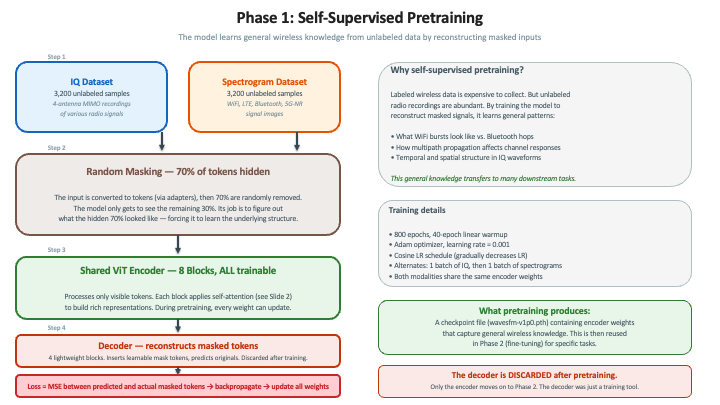
\includegraphics[width=\textwidth]{wavesfm_architecture/Slide1.png}
    \caption{Phase 1: Self-supervised pretraining. Unlabeled IQ and spectrogram data are randomly masked (70\% of tokens hidden). The encoder processes only visible tokens---with all weights trainable---and a lightweight decoder attempts to reconstruct the masked portions. The loss is mean squared error on masked positions. After 800 epochs, the decoder is discarded and only the encoder weights are kept, saved as the checkpoint file \texttt{wavesfm-v1p0.pth}.}
    \label{fig:pretraining}
\end{figure}

The encoder is made up of 8 transformer blocks stacked in sequence. Each block performs three operations on every token: self-attention, a feed-forward network, and layer normalization. Figure~\ref{fig:block_detail} breaks down what happens inside a single block.

\begin{figure}[H]
    \centering
    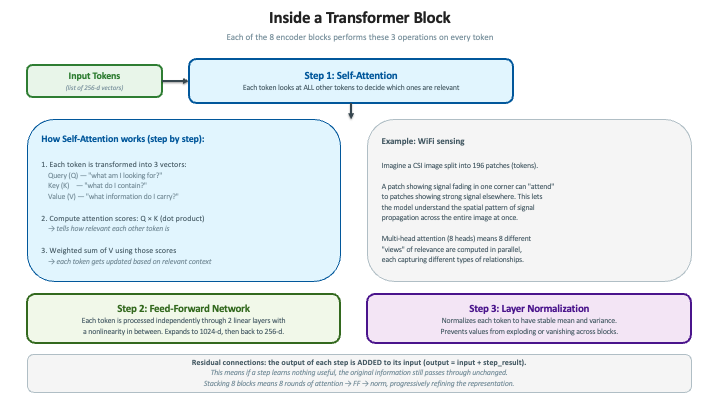
\includegraphics[width=\textwidth]{wavesfm_architecture/Slide2.png}
    \caption{Inside a transformer block. Step~1: Self-attention---each token examines all other tokens to find relevant context (e.g., a token from one antenna attending to tokens from other antennas to understand spatial patterns). Step~2: A feed-forward network processes each token independently, expanding from 256 to 1024 dimensions and back. Step~3: Layer normalization stabilizes the values. Residual connections add each step's output to its input, ensuring information flows even if a particular step learns nothing useful.}
    \label{fig:block_detail}
\end{figure}

The reconstruction loss that drives pretraining is mean squared error, computed only on the masked token positions:

\begin{equation}
\mathcal{L} = \frac{1}{|\mu_G|}\sum_{i \in \mu_G} \left\|\mathbf{x}_{i}^G - \hat{\mathbf{x}}_{i}^G\right\|^2 + \frac{1}{|\mu_Q|}\sum_{i \in \mu_Q} \left\|\mathbf{x}_{i}^Q - \hat{\mathbf{x}}_{i}^Q\right\|^2
\end{equation}

where $\mu_G$ and $\mu_Q$ are the sets of masked token indices for image-like and IQ inputs, respectively. Pretraining runs for 800 epochs with a 40-epoch warmup, using Adam optimizer with learning rate $10^{-3}$ and cosine annealing. The pretraining data consists of 3,200 spectrogram samples and 3,200 IQ samples~\cite{wavesfm_paper}.

\subsection{Model Size}

All published benchmarks use the \textbf{Small} configuration, summarized in Table~\ref{tab:model_config}. At roughly 7 million parameters total, this is a compact model. For context, the standard ViT-Base model from the original ViT paper~\cite{dosovitskiy2021vit} has 86 million parameters, and ViT-Large has 307 million---meaning WavesFM's encoder is roughly 12$\times$ smaller than ViT-Base.

\begin{table}[H]
\centering
\caption{WavesFM model configurations. All benchmarks use the Small variant.}
\label{tab:model_config}
\begin{tabular}{lccccc}
\toprule
 & \textbf{Embed Dim} & \textbf{Blocks} & \textbf{Heads} & \textbf{MLP Ratio} & \textbf{Params (M)} \\
\midrule
Micro  & 128 & 4  & 4  & 4.0 & --- \\
\textbf{Small}  & \textbf{256} & \textbf{8}  & \textbf{8}  & \textbf{4.0} & \textbf{6.32 (enc) + 0.79 (dec)} \\
Base   & 512 & 12 & 8  & 4.0 & --- \\
Large  & 768 & 12 & 12 & 4.0 & --- \\
\bottomrule
\end{tabular}
\end{table}

\subsection{Fine-Tuning: Reusing the Pretrained Encoder}

Once pretraining is complete, the encoder's learned weights are loaded and reused for specific downstream tasks. The fine-tuning pipeline chains together the same modality adapters and conditioning layer from pretraining, but now adds a task-specific head on top of the encoder. Figure~\ref{fig:finetuning_flow} shows this data flow end to end.

\begin{figure}[H]
    \centering
    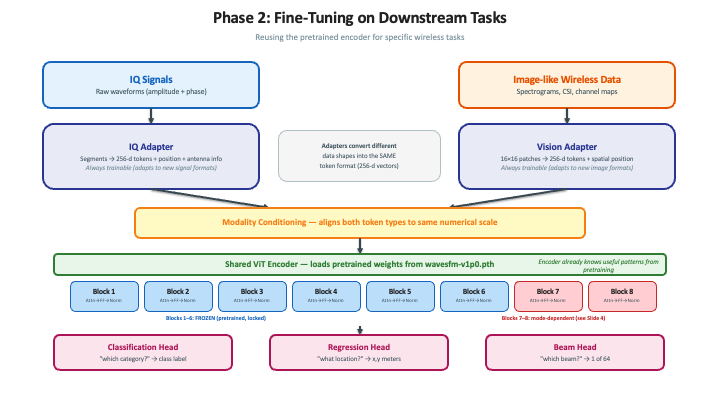
\includegraphics[width=\textwidth]{wavesfm_architecture/Slide3.png}
    \caption{Phase 2: Fine-tuning data flow. IQ signals and image-like data each pass through their respective adapters (which convert different data shapes into the same 256-d token format), then a modality conditioning layer, then the shared ViT encoder loaded with pretrained weights. Task-specific heads---classification, regression, or beam prediction---produce the final output.}
    \label{fig:finetuning_flow}
\end{figure}

The key question during fine-tuning is: how much of the pretrained encoder should be allowed to change? Allowing too much change risks losing the general knowledge learned during pretraining. Allowing too little may prevent the model from adapting to the new task. WavesFM evaluates three strategies, compared side by side in Figure~\ref{fig:three_modes}.

\begin{figure}[H]
    \centering
    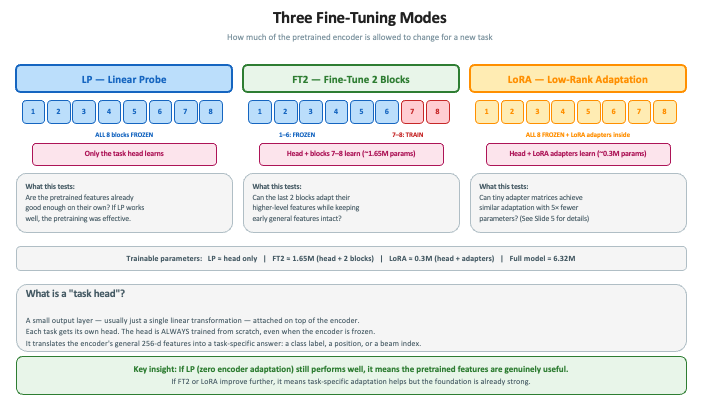
\includegraphics[width=\textwidth]{wavesfm_architecture/Slide4.png}
    \caption{The three fine-tuning modes. LP (Linear Probe) freezes all 8 encoder blocks and trains only the task head---testing whether the pretrained features are already useful. FT2 (Fine-Tune 2) freezes blocks 1--6 and allows blocks 7--8 to adapt ($\sim$1.65M trainable parameters). LoRA (Low-Rank Adaptation) keeps all blocks frozen but inserts small adapter matrices inside each ($\sim$0.3M parameters). The bottom section explains what a ``task head'' is: a single linear layer that translates the encoder's general features into a task-specific answer.}
    \label{fig:three_modes}
\end{figure}

Of the three modes, LoRA deserves special attention because of how it achieves adaptation without modifying the original weights. Instead of updating the full 256$\times$256 weight matrices inside each attention layer (65,536 parameters each), LoRA inserts two small matrices that squeeze the signal through a low-dimensional bottleneck. Figure~\ref{fig:lora_detail} walks through this mechanism step by step.

\begin{figure}[H]
    \centering
    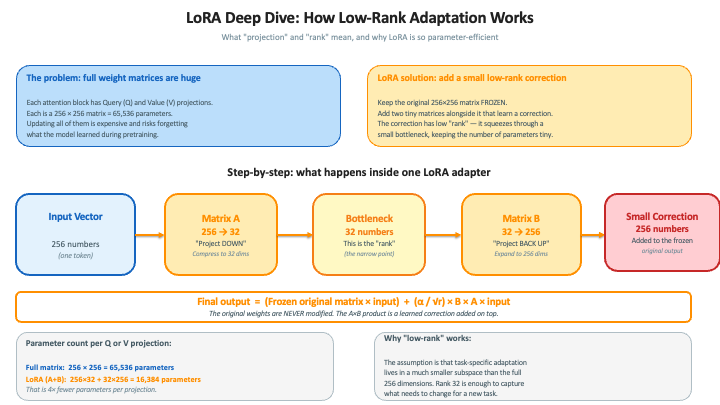
\includegraphics[width=\textwidth]{wavesfm_architecture/Slide5.png}
    \caption{LoRA deep dive. The original weight matrix stays frozen. Two small matrices are added alongside: Matrix~A projects the 256-dimensional input down to 32 dimensions (the ``rank''), and Matrix~B projects it back up to 256. The result is a small correction added to the frozen output. This requires only 16,384 parameters per projection instead of 65,536---a 4$\times$ reduction---yet achieves comparable adaptation to partial fine-tuning.}
    \label{fig:lora_detail}
\end{figure}

% ============================================================
%  4  Tasks and Metrics
% ============================================================
\section{Downstream Tasks and Evaluation Metrics}
\label{sec:tasks}

The WavesFM benchmark evaluates the pretrained model on 11 downstream tasks, listed in Table~\ref{tab:tasks}. This breadth is deliberate: a foundation model should work across many different problems, not just one.

\begin{table}[H]
\centering
\caption{The downstream tasks in the WavesFM benchmark, spanning two modality families and multiple application domains.}
\label{tab:tasks}
\small
\begin{tabular}{lp{2.5cm}p{4.5cm}rl}
\toprule
\textbf{Task ID} & \textbf{Modality} & \textbf{What It Does} & \textbf{Classes} & \textbf{Metric} \\
\midrule
\code{sensing}       & Vision (CSI)       & Recognizes human activities (walking, sitting, lying down, etc.) from WiFi signals & 6   & PCA \\
\code{rfs}           & Vision (spectrogram) & Classifies radio signal types (WiFi, FM, cellular, Bluetooth, etc.)~\cite{zahid2024commrad} & 20  & PCA \\
\code{pos}           & Vision (CSI)       & Estimates a device's physical location from 5G channel measurements & ---  & Mean error \\
\code{radcom}        & IQ                 & Classifies modulation and signal type from over-the-air captures & 9   & PCA \\
\code{uwb-indoor}    & IQ (CIR)           & Locates objects indoors using ultra-wideband radio pulses & ---  & Mean error \\
\code{uwb-industrial}& IQ (CIR)           & Locates objects in industrial environments using UWB & ---  & Mean error \\
\code{rml}           & IQ                 & Identifies modulation type (QPSK, QAM, etc.) from raw signals & 11  & PCA \\
\code{rfp}           & IQ                 & Identifies which specific device transmitted a signal (RF fingerprinting) & 4   & PCA \\
\code{interf}        & IQ                 & Detects and classifies radio interference & 3   & PCA \\
\code{deepmimo-los}  & Vision (channel)   & Determines if a signal has a direct path (line-of-sight) or not & 2   & PCA \\
\code{deepmimo-beam} & Vision (channel)   & Predicts the best antenna beam direction for communication & 64  & PCA \\
\bottomrule
\end{tabular}
\end{table}

\subsection{Metrics}

\paragraph{Per-Class Accuracy (PCA).} The primary metric for all classification tasks. PCA computes accuracy separately for each class and then averages across classes. This is more informative than regular accuracy when some classes have far more samples than others, because it treats every class as equally important. For example, if a dataset has 90\% of samples in class~A and 10\% in class~B, a model that always predicts class~A would achieve 90\% regular accuracy but only 50\% PCA.

\paragraph{Mean Distance Error.} The primary metric for positioning tasks. It measures the average Euclidean distance (in meters) between the model's predicted location and the true location. Lower values indicate better performance.

\paragraph{Checkpoint Selection.} During training, the model is evaluated on a held-out validation set after each epoch. The checkpoint with the best validation metric is kept as the final model---highest PCA for classification, lowest mean error for regression.

% ============================================================
%  5  Reproduction Methodology
% ============================================================
\section{Reproduction Methodology}
\label{sec:methodology}

\subsection{Starting Point}

The reproduction began with the publicly available artifacts from the WavesFM project:
\begin{itemize}
    \item The code repository, containing the model definition, training scripts, and preprocessing pipelines
    \item The pretrained checkpoint (\code{wavesfm-v1p0.pth}), containing the model weights after self-supervised pretraining
    \item Dataset documentation on the WavesFM website~\cite{wavesfm_home}, with links to raw data sources
    \item The official reproduce page~\cite{wavesfm_reproduce}, recommending Python 3.10+, PyTorch 2.x with CUDA, and a GPU comparable to an NVIDIA A100
\end{itemize}

\subsection{Acquiring and Preprocessing the Datasets}

Each task requires a specific raw dataset that must be downloaded from its public source and converted into an HDF5 cache file (a compact binary format optimized for fast loading during training). The WavesFM repository includes preprocessing scripts for each task. Table~\ref{tab:data_status} shows the acquisition status.

\begin{table}[H]
\centering
\caption{Dataset acquisition status for each task.}
\label{tab:data_status}
\small
\begin{tabular}{lp{5.8cm}l}
\toprule
\textbf{Task} & \textbf{Raw Data Source} & \textbf{Status} \\
\midrule
\code{sensing}        & NTU-Fi HAR WiFi CSI \code{.mat} files        & Ready \\
\code{pos}            & IEEE Dataport 5G NR CSI measurements         & Ready \\
\code{radcom}         & RadCom OTA HDF5 signal captures              & Ready \\
\code{rml}            & RadioML 2022 modulation samples               & Ready \\
\code{rfp}            & POWDER PAWR platform IQ fingerprints          & Ready \\
\code{uwb-indoor}     & UWB indoor CIR data (4 environments)          & Ready (after bug fix) \\
\code{uwb-industrial} & Industrial UWB localization data               & Ready \\
\code{interf}         & ICARUS interference IQ recordings              & Ready \\
\code{deepmimo}       & DeepMIMO scenario channel data via DeepMIMOv3  & Ready (rebuilt twice) \\
\code{lwm-beam}       & LWM beam-challenge pickle files                & Ready (hypothesis only) \\
\code{rfs}            & CommRad archive (\code{.wav} recordings)       & \textbf{Blocked}---format mismatch \\
\bottomrule
\end{tabular}
\end{table}

The \code{rfs} task could not proceed because the publicly available data (nested folders of \code{.wav} audio files labeled by radio device) does not match what the preprocessing script expects (a flat folder of spectrogram images labeled by signal type). The label semantics are fundamentally different, so no faithful reproduction was possible.

\subsection{Hardware: MacBook Pro, Then Lab Server}
\label{subsec:hardware}

Development started on a \textbf{MacBook Pro}, which was practical for code inspection, dataset acquisition, preprocessing, and documentation. The released code assumed NVIDIA CUDA hardware, so it was adapted for Apple's MPS GPU backend. Even with this adaptation, training was too slow for the full benchmark---10 tasks $\times$ 3 fine-tuning modes $\times$ 3 random seeds = 90 individual training runs.

The benchmarking was therefore moved to a \textbf{university lab Linux server} (\code{ngwn06}):
\begin{itemize}
    \item \textbf{GPU:} NVIDIA GeForce RTX 5090
    \item \textbf{CPU:} 24 cores, 62\,GB RAM
    \item \textbf{Software:} PyTorch 2.9.1, CUDA 12.4, timm 1.0.11, h5py 3.15.1
\end{itemize}

The MacBook remained the canonical editing environment. Code changes were made locally and synced to the server via \code{rsync}; results were synced back after each session. Long-running experiments were launched in \code{tmux} sessions to continue unattended.

\subsection{Code Modifications}
\label{subsec:code_changes}

Running the released code required several modifications, categorized by impact:

\paragraph{Bug fixes (the code would not run without these).}
\begin{itemize}
    \item One script imported a module that does not exist in the release, crashing at startup.
    \item The UWB indoor preprocessing script referenced a command-line argument that was never defined.
\end{itemize}

\paragraph{Hardware adaptations (no effect on scientific results).}
\begin{itemize}
    \item Replaced hard-coded \code{cuda} device with automatic selection (CUDA $\rightarrow$ Apple MPS $\rightarrow$ CPU).
    \item Restricted mixed-precision training features to CUDA only (unsupported on Apple GPUs).
    \item Added crash-recovery hardening: atomic checkpoint saves, RNG state preservation, and fsynced logging.
\end{itemize}

\paragraph{Benchmark protocol changes (may affect results for specific tasks).}
\begin{itemize}
    \item Changed the DeepMIMO beam codebook from 16 to 64 beams to match the public WavesFM setup.
    \item Fixed a bug in the beam angle sweep that duplicated one endpoint and left the highest beam class unreachable (changed from inclusive $[-90^{\circ}, +90^{\circ}]$ to half-open $[-90^{\circ}, 90^{\circ})$).
    \item Adjusted the model's output layer to match the full 64-beam codebook rather than the number of labels observed in the data.
    \item Added a separate experimental task (\code{lwm-beam-challenge}) for hypothesis testing, kept isolated from the official benchmark pipeline.
\end{itemize}

A full code change log is provided in Appendix~\ref{app:code_changes}.

\subsection{Training Configuration}

Every task was trained using the hyperparameters specified in the WavesFM benchmark configuration, summarized in Table~\ref{tab:hyperparams}. All tasks shared the same optimizer (AdamW with weight decay 0.05), learning rate schedule (cosine annealing from $10^{-3}$ down to $10^{-6}$, with a 5-epoch warmup), and layer-wise learning rate decay (factor 0.75).

\begin{table}[H]
\centering
\caption{Task-specific training hyperparameters.}
\label{tab:hyperparams}
\small
\begin{tabular}{lcccc}
\toprule
\textbf{Task} & \textbf{Batch Size} & \textbf{Epochs} & \textbf{Label Smoothing} & \textbf{Notes} \\
\midrule
\code{sensing}            & 256  & 100 & 0.10 & Stratified split \\
\code{pos}                & 256  & 100 & ---  & --- \\
\code{radcom}             & 2048 & 50  & ---  & --- \\
\code{uwb-indoor}         & 256  & 50  & ---  & --- \\
\code{uwb-industrial}     & 512  & 50  & ---  & --- \\
\code{rml}                & 2048 & 50  & ---  & --- \\
\code{rfp}                & 256  & 10  & 0.10 & --- \\
\code{interf}             & 256  & 35  & 0.02 & Stratified split, class weights \\
\code{deepmimo-los}       & 256  & 100 & ---  & Stratified split, class weights \\
\code{deepmimo-beam}      & 256  & 100 & ---  & Stratified split, class weights \\
\bottomrule
\end{tabular}
\end{table}

Each task/mode combination was run with three different random seeds (0, 1, 2) and the results averaged, following the official protocol. This ensures that results reflect genuine model behavior rather than a lucky initialization.

\subsection{Three Experimental Sessions}

Three sessions were conducted, each building on findings from the previous one:

\begin{enumerate}
    \item \textbf{First full run} (April 3, 2026): All 10 available tasks, 3 modes each, 3 seeds = \textbf{90 runs}. This provided baseline results for every task.

    \item \textbf{Corrected second pass} (April 15, 2026): Reran \code{sensing}, \code{deepmimo-los}, and \code{deepmimo-beam} after discovering and fixing the beam codebook bug. \textbf{27 runs}. These replaced the first-pass results for those three tasks.

    \item \textbf{Hypothesis test} (April 15, 2026): Ran the \code{lwm-beam-challenge} experiment to investigate the beam prediction discrepancy. \textbf{9 runs}. This was a diagnostic experiment, not a benchmark reproduction.
\end{enumerate}

Each session produced training logs, model checkpoints, summary statistics, local-vs-official comparison files, and visualization plots (confusion matrices for classification tasks, error density plots for positioning tasks).


% ============================================================
%  6  Official Baselines
% ============================================================
\section{Official Baseline Results}
\label{sec:official}

The official results were obtained from the WavesFM detailed evaluation page~\cite{wavesfm_detailed_eval} and stored locally as a JSON snapshot (dated January 23, 2026). These are the target values the reproduction aimed to match.

\begin{table}[H]
\centering
\caption{{\color{officialblue}Official} WavesFM classification results (PCA \%, higher is better).}
\label{tab:official_cls}
\begin{tabular}{l >{\columncolor{officialbg}}c >{\columncolor{officialbg}}c >{\columncolor{officialbg}}c}
\toprule
\textbf{Task} & {\color{officialblue}\textbf{LP}} & {\color{officialblue}\textbf{FT2}} & {\color{officialblue}\textbf{LoRA}} \\
\midrule
\code{sensing}        & 94.42 & 99.31 & 98.47 \\
\code{rfs}            & 42.85 & 83.41 & 84.49 \\
\code{radcom}         & 90.10 & 94.53 & 93.78 \\
\code{rml}            & 50.39 & 55.16 & 56.49 \\
\code{rfp}            & 98.97 & 99.70 & 99.82 \\
\code{interf}         & 71.50 & 78.94 & 78.94 \\
\code{deepmimo-los}   & 95.02 & 95.46 & 95.24 \\
\code{deepmimo-beam}  & 67.67 & 78.38 & 77.38 \\
\bottomrule
\end{tabular}
\end{table}

\begin{table}[H]
\centering
\caption{{\color{officialblue}Official} WavesFM regression results (mean distance error in meters, lower is better).}
\label{tab:official_reg}
\begin{tabular}{l >{\columncolor{officialbg}}c >{\columncolor{officialbg}}c >{\columncolor{officialbg}}c}
\toprule
\textbf{Task} & {\color{officialblue}\textbf{LP}} & {\color{officialblue}\textbf{FT2}} & {\color{officialblue}\textbf{LoRA}} \\
\midrule
\code{pos}             & 3.17 & 1.24 & 1.45 \\
\code{uwb-indoor}      & 1.43 & 0.83 & 0.65 \\
\code{uwb-industrial}  & 2.71 & 0.88 & 0.74 \\
\bottomrule
\end{tabular}
\end{table}


% ============================================================
%  7  Results
% ============================================================
\section{Reproduction Results}
\label{sec:results}

\subsection{The Full Picture}

Table~\ref{tab:full_results} presents all 30 task/mode results alongside the official baselines. For \code{sensing}, \code{deepmimo-los}, and \code{deepmimo-beam}, the numbers come from the corrected second pass; for all other tasks, they come from the first full run.

\begin{landscape}
\begin{table}
\centering
\caption{Complete reproduction results. {\color{officialblue}\textbf{Blue}} = official published values; {\color{localgreen}\textbf{green}} = local reproduction. Classification: PCA (\%); regression: mean error in meters. ``$\Delta$'' = local $-$ official (for classification, positive means the local result was higher; for regression, negative means the local error was lower). Superscripts: \textsuperscript{1}first run, \textsuperscript{2}corrected second pass.}
\label{tab:full_results}
\small
\begin{tabular}{l l >{\columncolor{officialbg}}c >{\columncolor{localbg}}c c >{\columncolor{officialbg}}c >{\columncolor{localbg}}c c >{\columncolor{officialbg}}c >{\columncolor{localbg}}c c l}
\toprule
& & \multicolumn{3}{c}{\textbf{Linear Probe (LP)}} & \multicolumn{3}{c}{\textbf{Fine-Tune 2 (FT2)}} & \multicolumn{3}{c}{\textbf{LoRA}} & \\
\cmidrule(lr){3-5} \cmidrule(lr){6-8} \cmidrule(lr){9-11}
\textbf{Task} & \textbf{Unit} & {\color{officialblue}\textbf{Official}} & {\color{localgreen}\textbf{Local}} & \textbf{$\Delta$} & {\color{officialblue}\textbf{Official}} & {\color{localgreen}\textbf{Local}} & \textbf{$\Delta$} & {\color{officialblue}\textbf{Official}} & {\color{localgreen}\textbf{Local}} & \textbf{$\Delta$} & \textbf{Verdict} \\
\midrule
\code{rfp}\textsuperscript{1}    & \% & 98.97 & 98.98 & $+$0.01  & 99.70 & 99.70 & $\approx$0  & 99.82 & 99.84 & $+$0.02  & Reproduced \\
\code{rml}\textsuperscript{1}    & \% & 50.39 & 50.39 & $\approx$0  & 55.16 & 55.14 & $-$0.02  & 56.49 & 56.42 & $-$0.07  & Reproduced \\
\code{radcom}\textsuperscript{1} & \% & 90.10 & 90.12 & $+$0.02  & 94.53 & 94.61 & $+$0.08  & 93.78 & 94.07 & $+$0.29  & Reproduced \\
\code{interf}\textsuperscript{1} & \% & 71.50 & 71.17 & $-$0.33  & 78.94 & 78.83 & $-$0.11  & 78.94 & 79.67 & $+$0.73  & Reproduced \\
\code{d.mimo-los}\textsuperscript{2} & \% & 95.02 & 95.12 & $+$0.10  & 95.46 & 95.36 & $-$0.10  & 95.24 & 95.16 & $-$0.08  & Reproduced \\
\midrule
\code{pos}\textsuperscript{1}    & m   & 3.17 & 3.14  & $-$0.03  & 1.24 & 1.26  & $+$0.02  & 1.45 & 1.51 & $+$0.06  & Reproduced \\
\code{uwb-in}\textsuperscript{1} & m & 1.43 & 1.44 & $+$0.01  & 0.83 & 0.82 & $-$0.01  & 0.65 & 0.65 & $\approx$0  & Reproduced \\
\code{uwb-ind}\textsuperscript{1}& m & 2.71 & 2.71 & $\approx$0  & 0.88 & 0.88 & $\approx$0  & 0.74 & 0.74 & $\approx$0  & Reproduced \\
\midrule
\code{sensing}\textsuperscript{2} & \% & 94.42 & 93.89 & $-$0.53  & 99.31 & 98.47 & $-$0.84  & 98.47 & 99.31 & $+$0.84  & Close (caveat) \\
\midrule
\code{d.mimo-beam}\textsuperscript{2} & \% & 67.67 & {\color{gapred}56.37} & {\color{gapred}$-$11.30}  & 78.38 & {\color{gapred}69.44} & {\color{gapred}$-$8.94}  & 77.38 & {\color{gapred}67.84} & {\color{gapred}$-$9.54}  & \textbf{Not reproduced} \\
\code{rfs}          & \% & 42.85 & --- & ---  & 83.41 & --- & ---  & 84.49 & --- & ---  & \textbf{Blocked} \\
\bottomrule
\end{tabular}
\end{table}
\end{landscape}

\subsection{Eight Tasks That Reproduced Successfully}

The strongest finding of this study is that \textbf{eight of ten attempted tasks reproduced within a fraction of a percentage point}. These span both modality families (vision and IQ) and both task types (classification and regression), confirming that the pretrained checkpoint transfers across diverse wireless problems.

Notable results:
\begin{itemize}
    \item \textbf{RF Fingerprinting}: The LoRA result (99.84\%) differs from official (99.82\%) by 0.02 percentage points. The standard deviation across seeds was only 0.01\%, making this the most precisely reproduced task.

    \item \textbf{Modulation Classification}: The LP result matched the official value to three decimal places (50.393\% vs.\ 50.39\%).

    \item \textbf{UWB Industrial}: All three modes matched within 0.004 meters---effectively identical.

    \item \textbf{5G NR Positioning}: All modes within 0.06 meters of official values.

    \item \textbf{DeepMIMO LoS/NLoS}: All modes within 0.10 percentage points after the corrected second pass. This is important because the same dataset and preprocessor are used for the beam prediction task (Section~\ref{subsec:beam}), demonstrating that the pipeline works correctly.
\end{itemize}

\vspace{0.3cm}
\noindent\fbox{\parbox{0.97\textwidth}{\small\textbf{How to read the plots below:} Each plot header contains two rows of numbers. The row labeled ``\textbf{Local}'' shows the {\color{localgreen}\textbf{reproduced metrics}} and the row labeled ``\textbf{Official}'' shows the {\color{officialblue}\textbf{published baseline metrics}}. Comparing these two rows shows how close the reproduction is to the original.

The \textbf{confusion matrix} or \textbf{error density curve} below the header visualizes the local reproduction in detail. In confusion matrices, diagonal cells show correct predictions (darker = more correct). In density curves, the shaded area shows the error distribution and the dashed red line marks the mean error. Official visualizations were not available---only the official metric values in the header.}}
\vspace{0.3cm}

\begin{figure}[H]
    \centering
    \begin{subfigure}[b]{0.48\textwidth}
        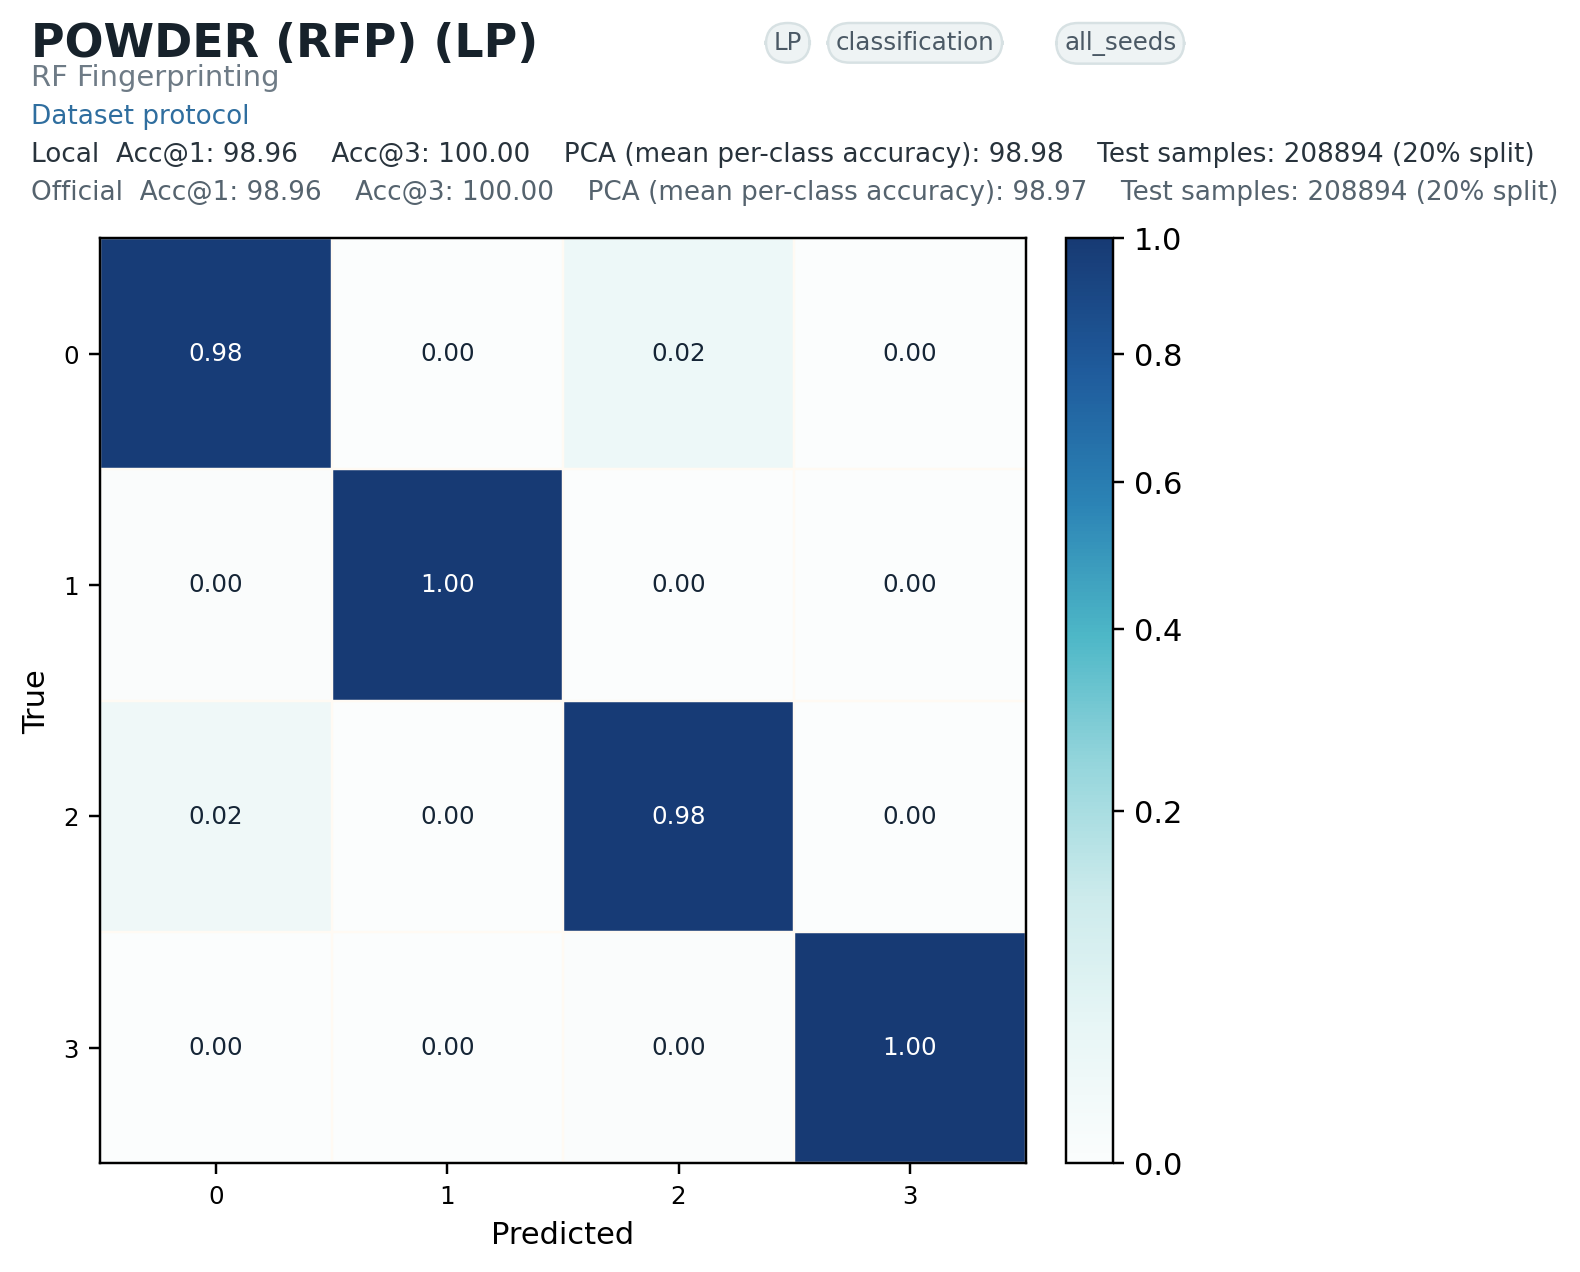
\includegraphics[width=\textwidth]{rfp_lp_cm.png}
        \caption{RFP -- LP}
    \end{subfigure}
    \begin{subfigure}[b]{0.48\textwidth}
        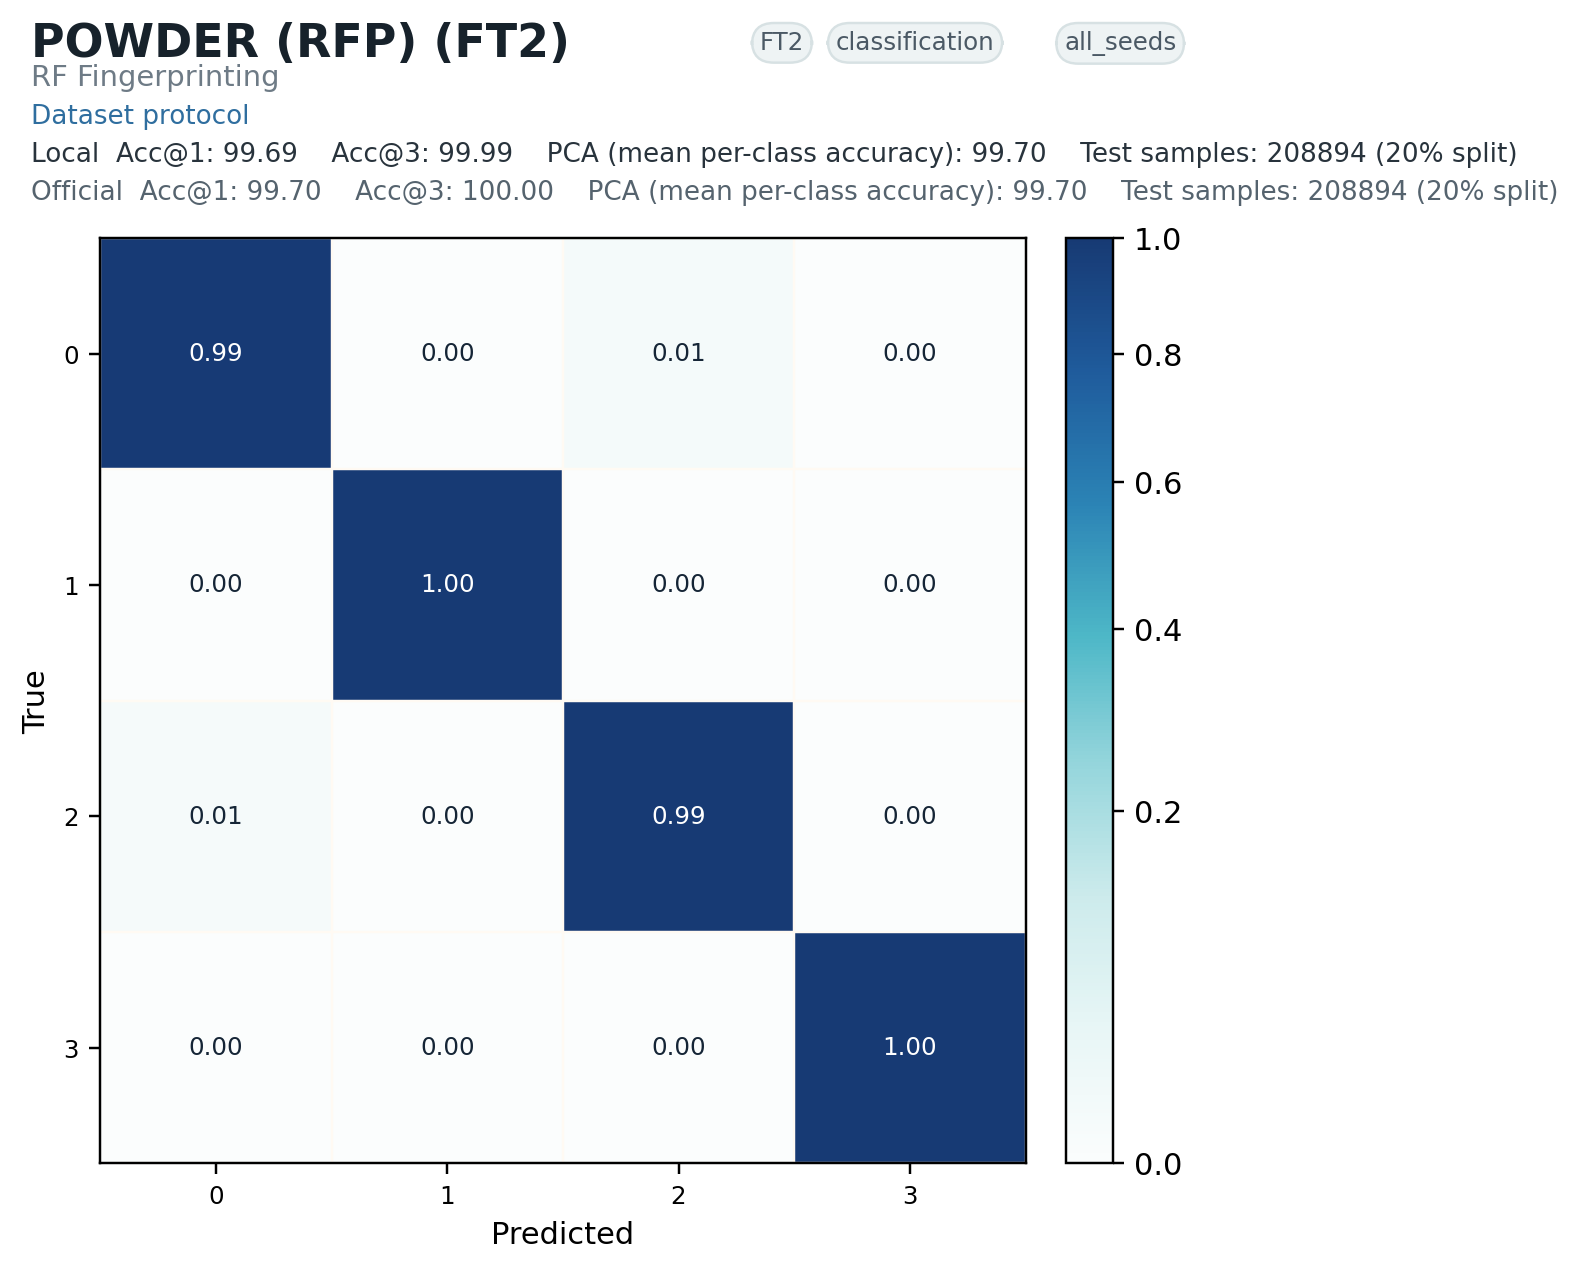
\includegraphics[width=\textwidth]{rfp_ft2_cm.png}
        \caption{RFP -- FT2}
    \end{subfigure}
    \begin{subfigure}[b]{0.48\textwidth}
        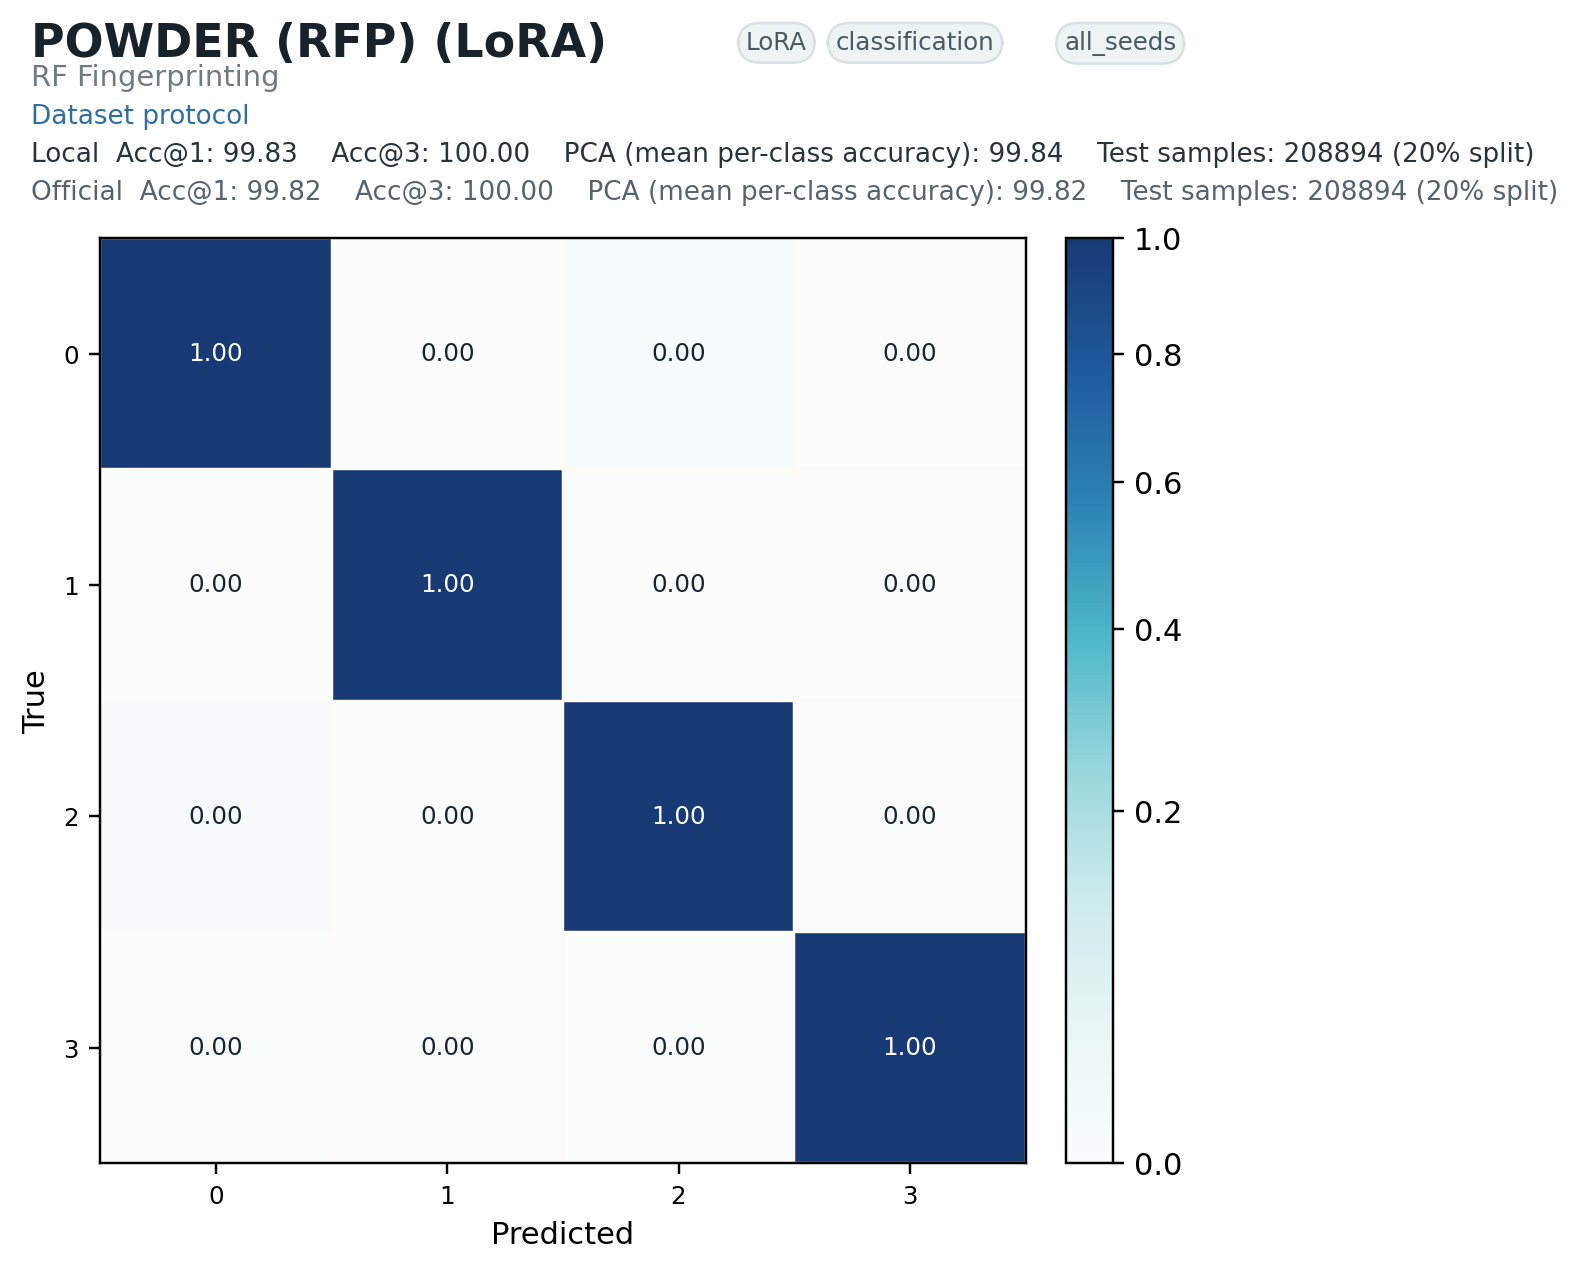
\includegraphics[width=\textwidth]{rfp_lora_cm.png}
        \caption{RFP -- LoRA}
    \end{subfigure}
    \caption{Confusion matrices for RF Fingerprinting (4 device classes). The near-perfect diagonal reflects $>$99\% PCA across all modes.}
    \label{fig:rfp_cm}
\end{figure}

\begin{figure}[H]
    \centering
    \begin{subfigure}[b]{0.48\textwidth}
        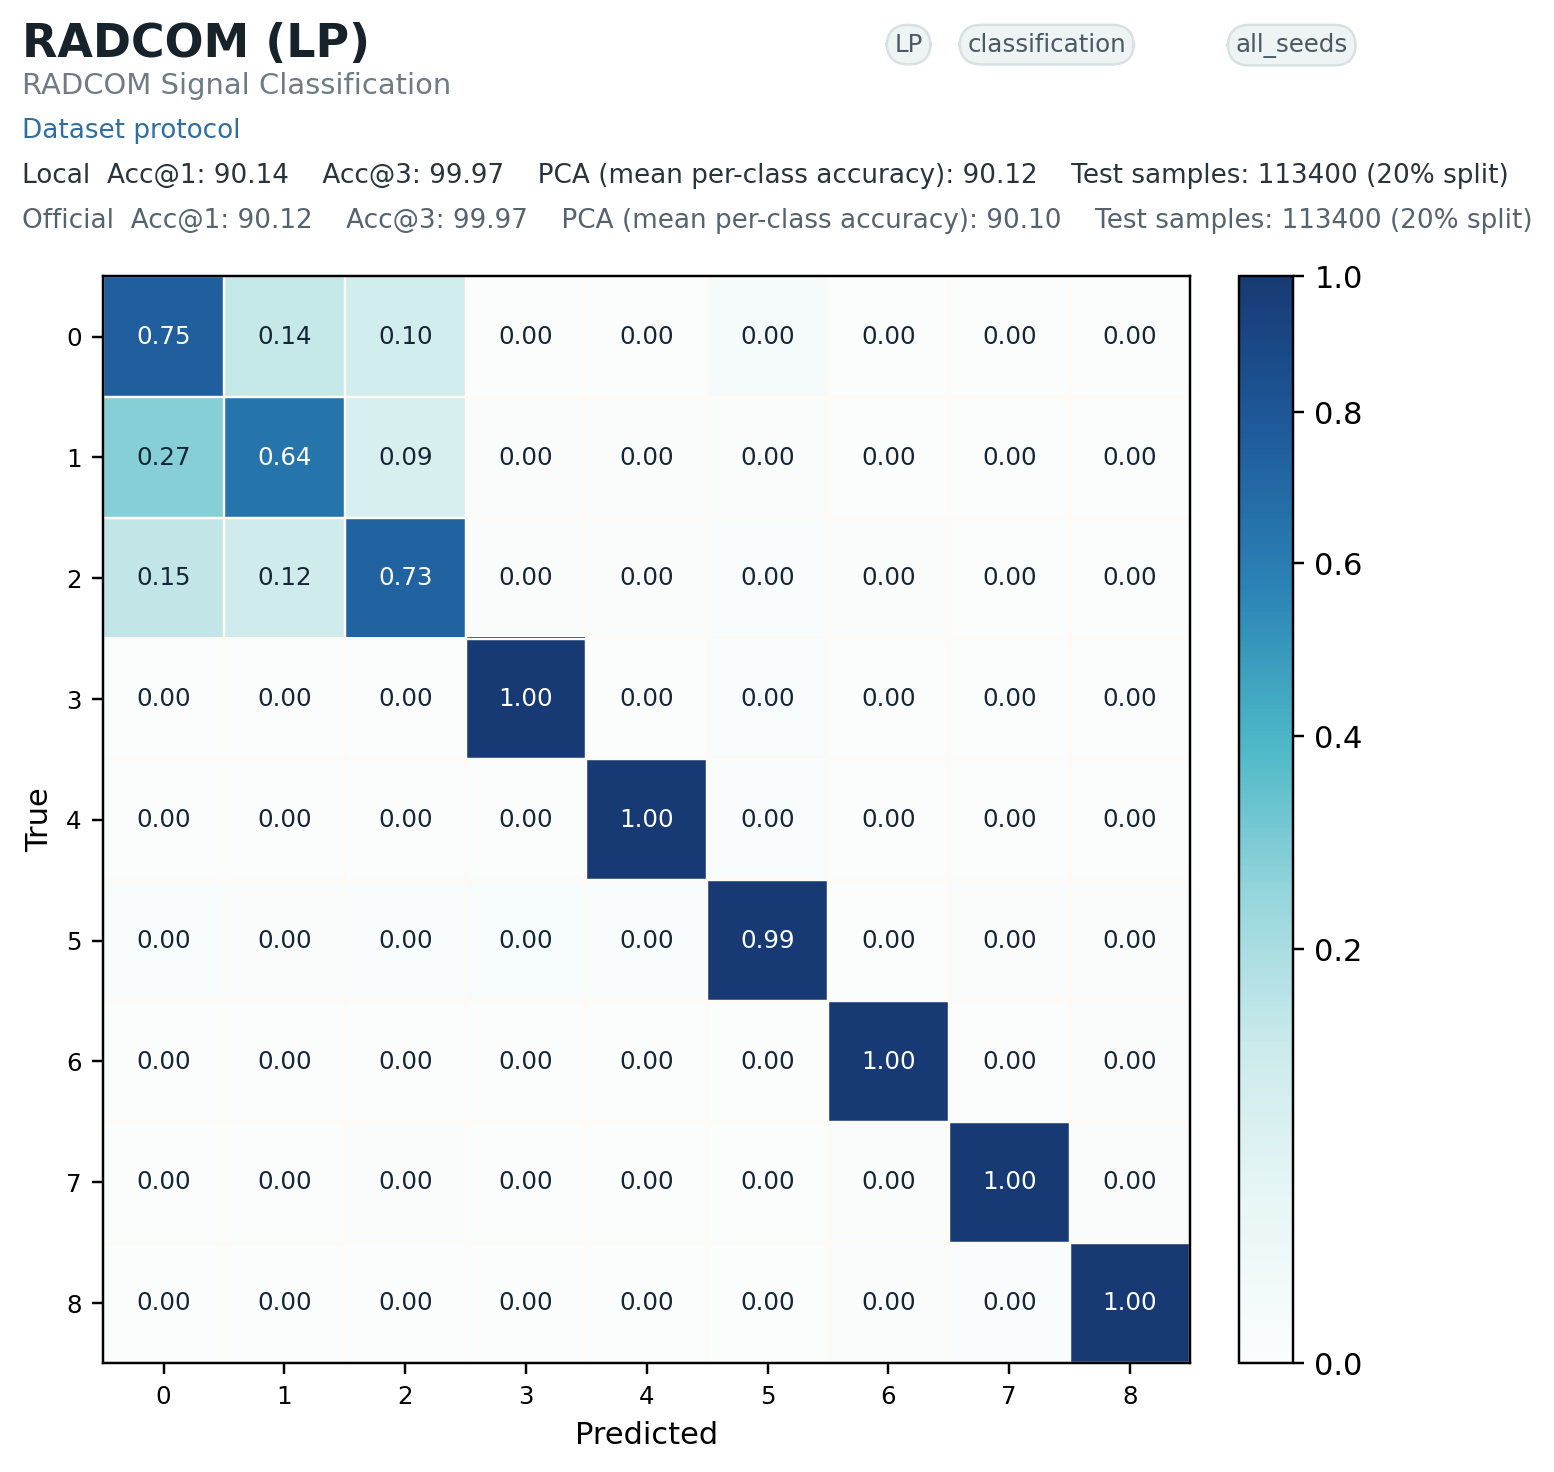
\includegraphics[width=\textwidth]{radcom_lp_cm.png}
        \caption{RADCOM -- LP}
    \end{subfigure}
    \begin{subfigure}[b]{0.48\textwidth}
        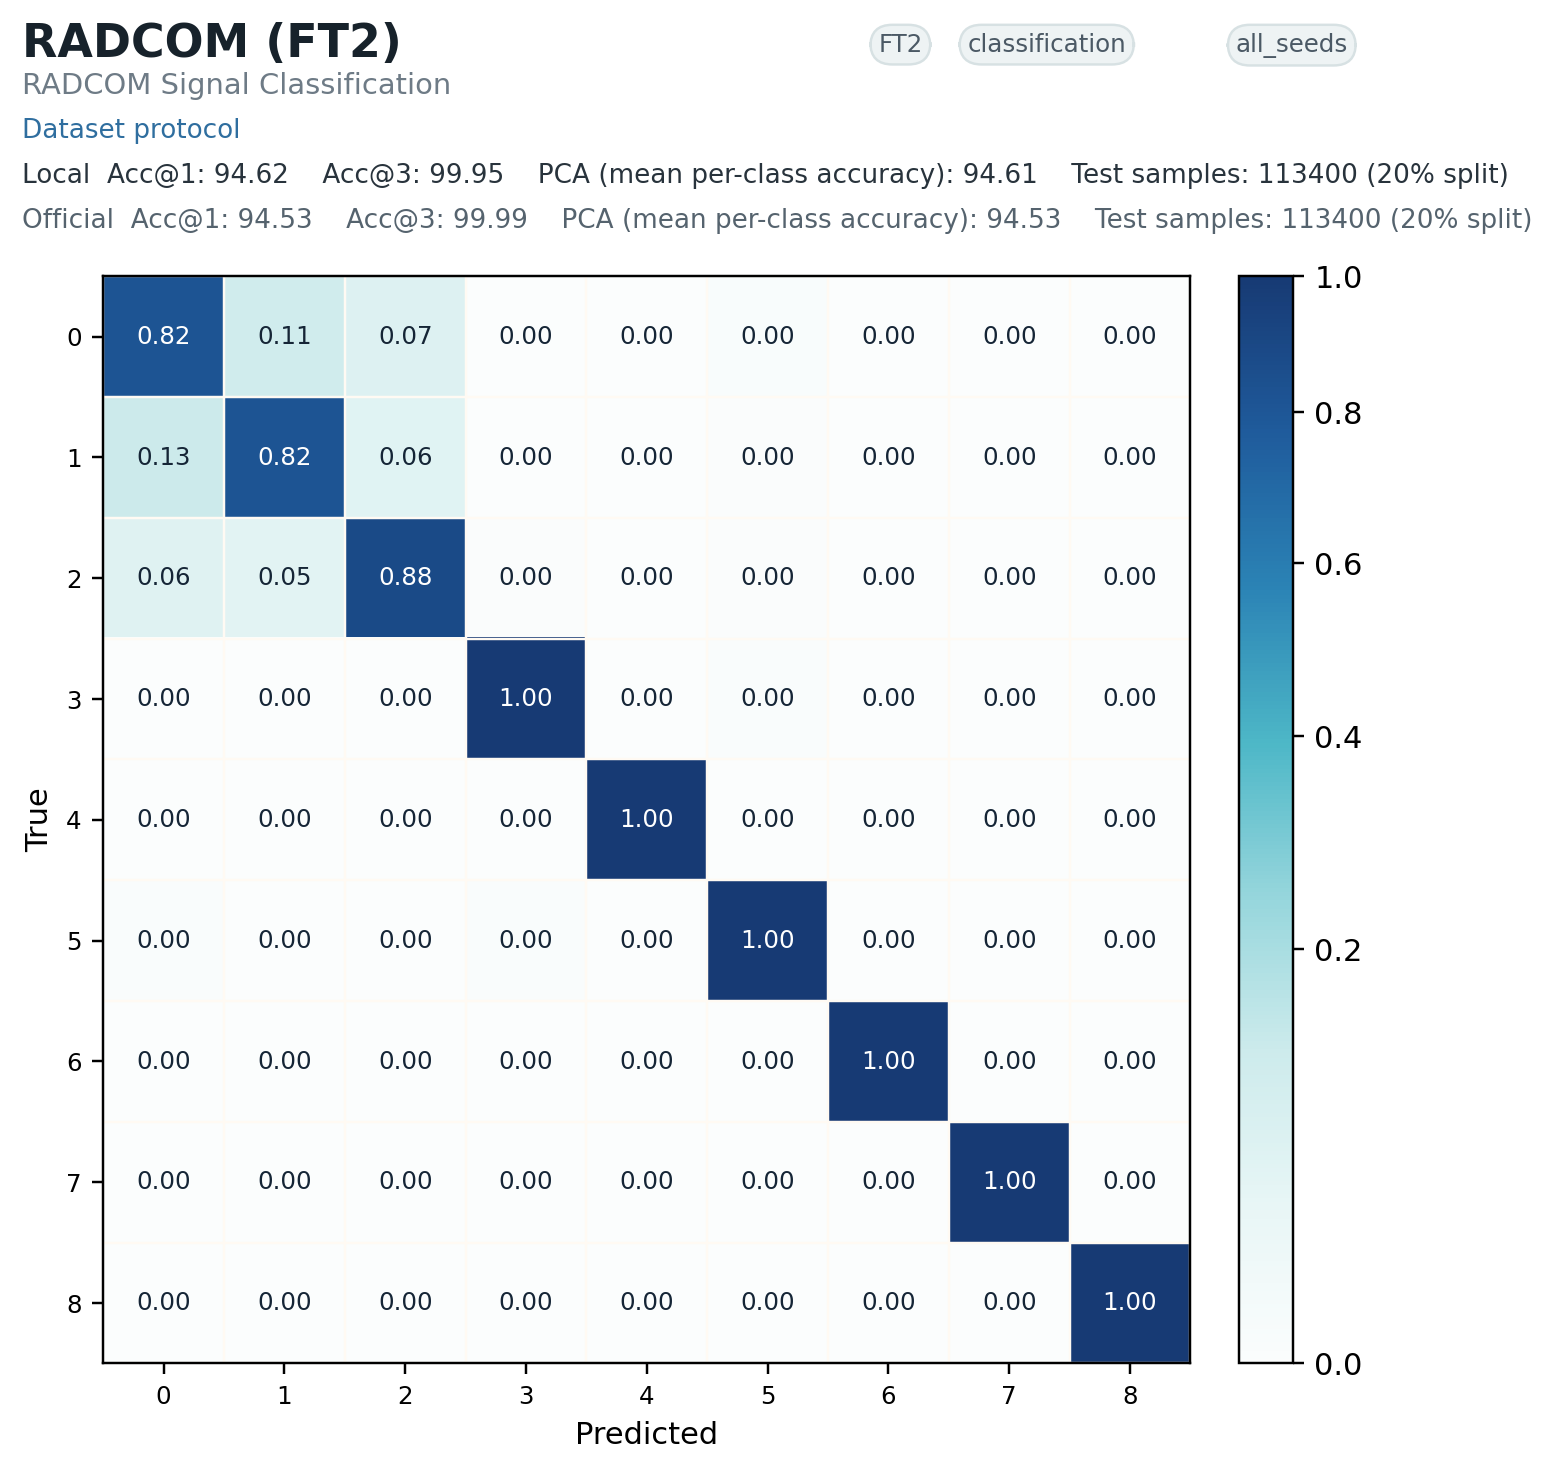
\includegraphics[width=\textwidth]{radcom_ft2_cm.png}
        \caption{RADCOM -- FT2}
    \end{subfigure}
    \begin{subfigure}[b]{0.48\textwidth}
        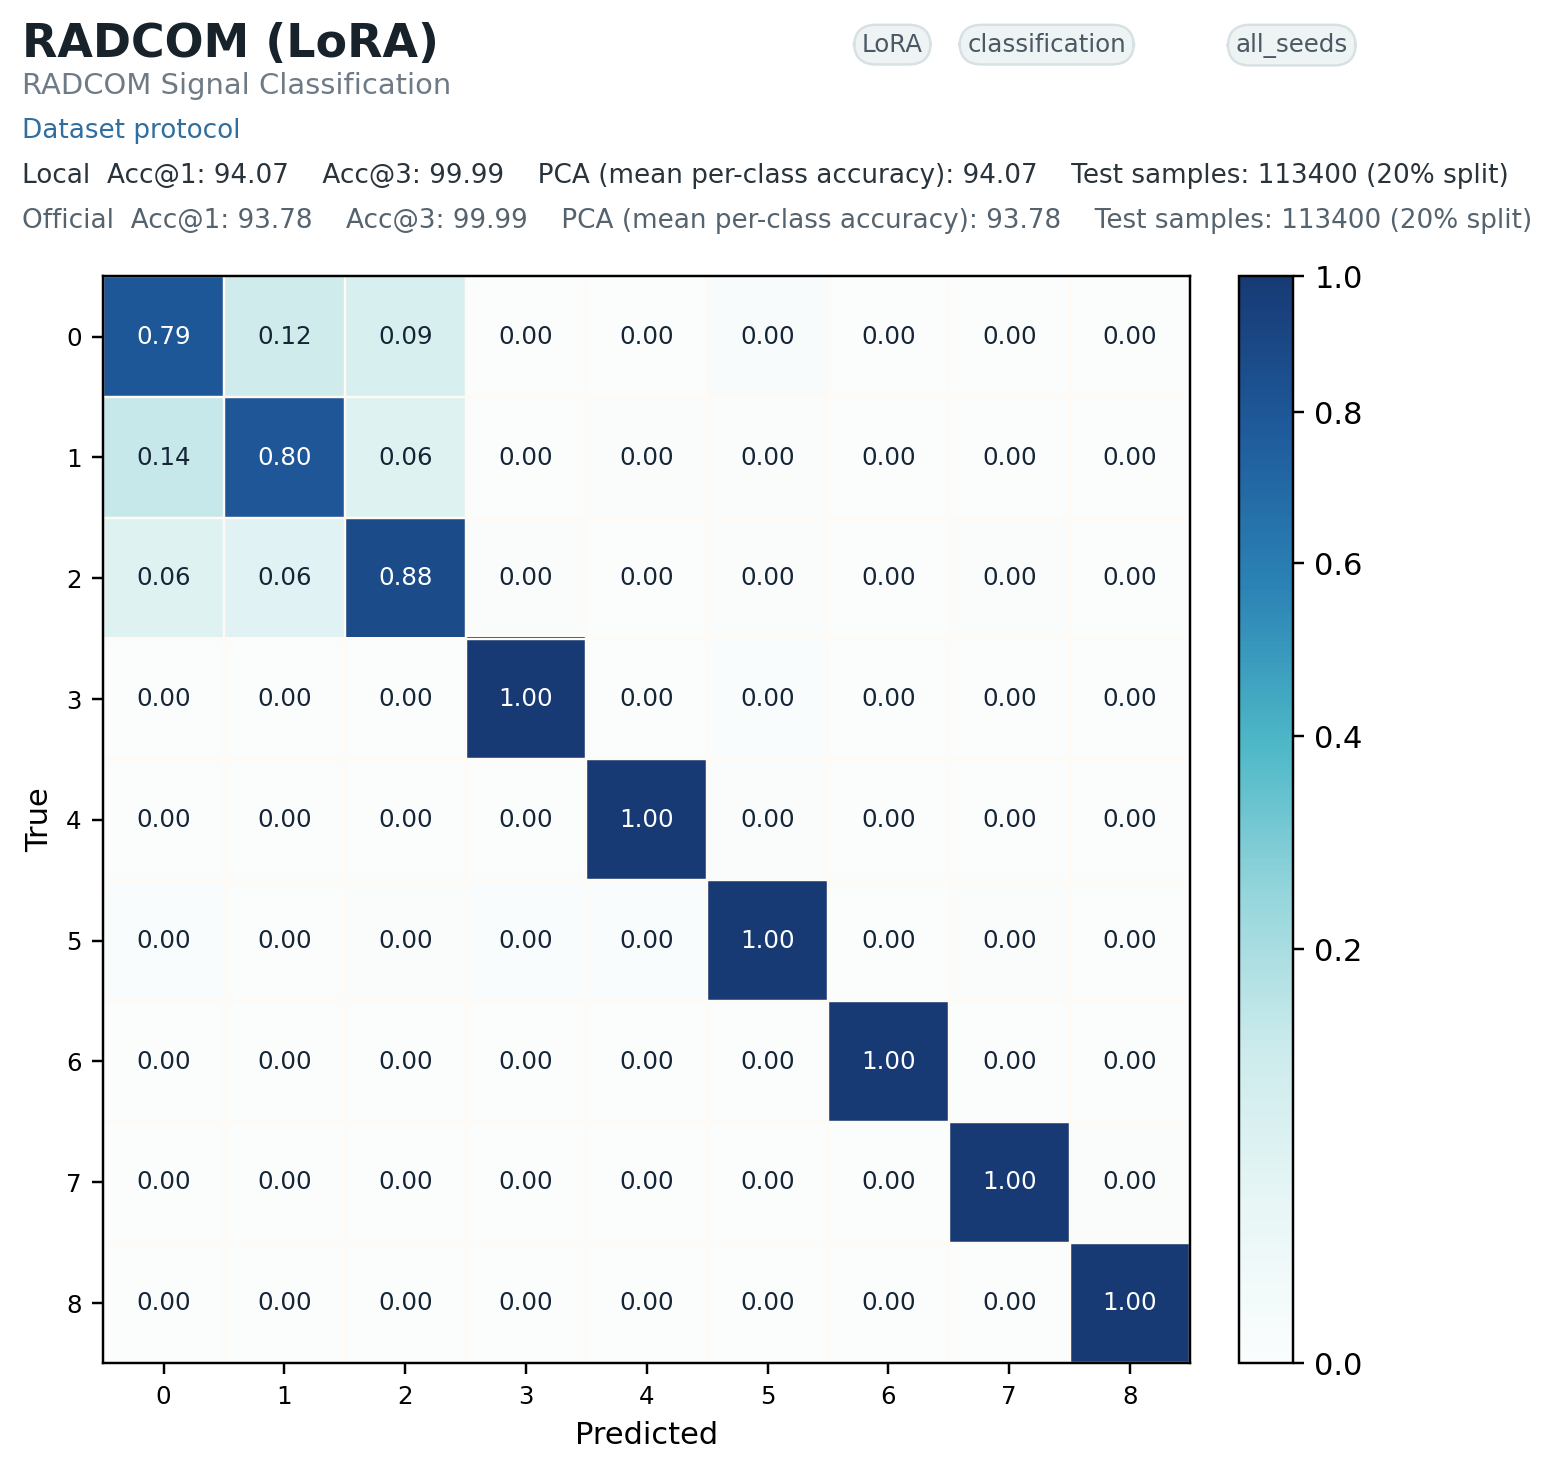
\includegraphics[width=\textwidth]{radcom_lora_cm.png}
        \caption{RADCOM -- LoRA}
    \end{subfigure}
    \caption{Confusion matrices for RADCOM signal classification (9 classes). Off-diagonal entries indicate misclassifications between similar signal types.}
    \label{fig:radcom_cm}
\end{figure}

\begin{figure}[H]
    \centering
    \begin{subfigure}[b]{0.48\textwidth}
        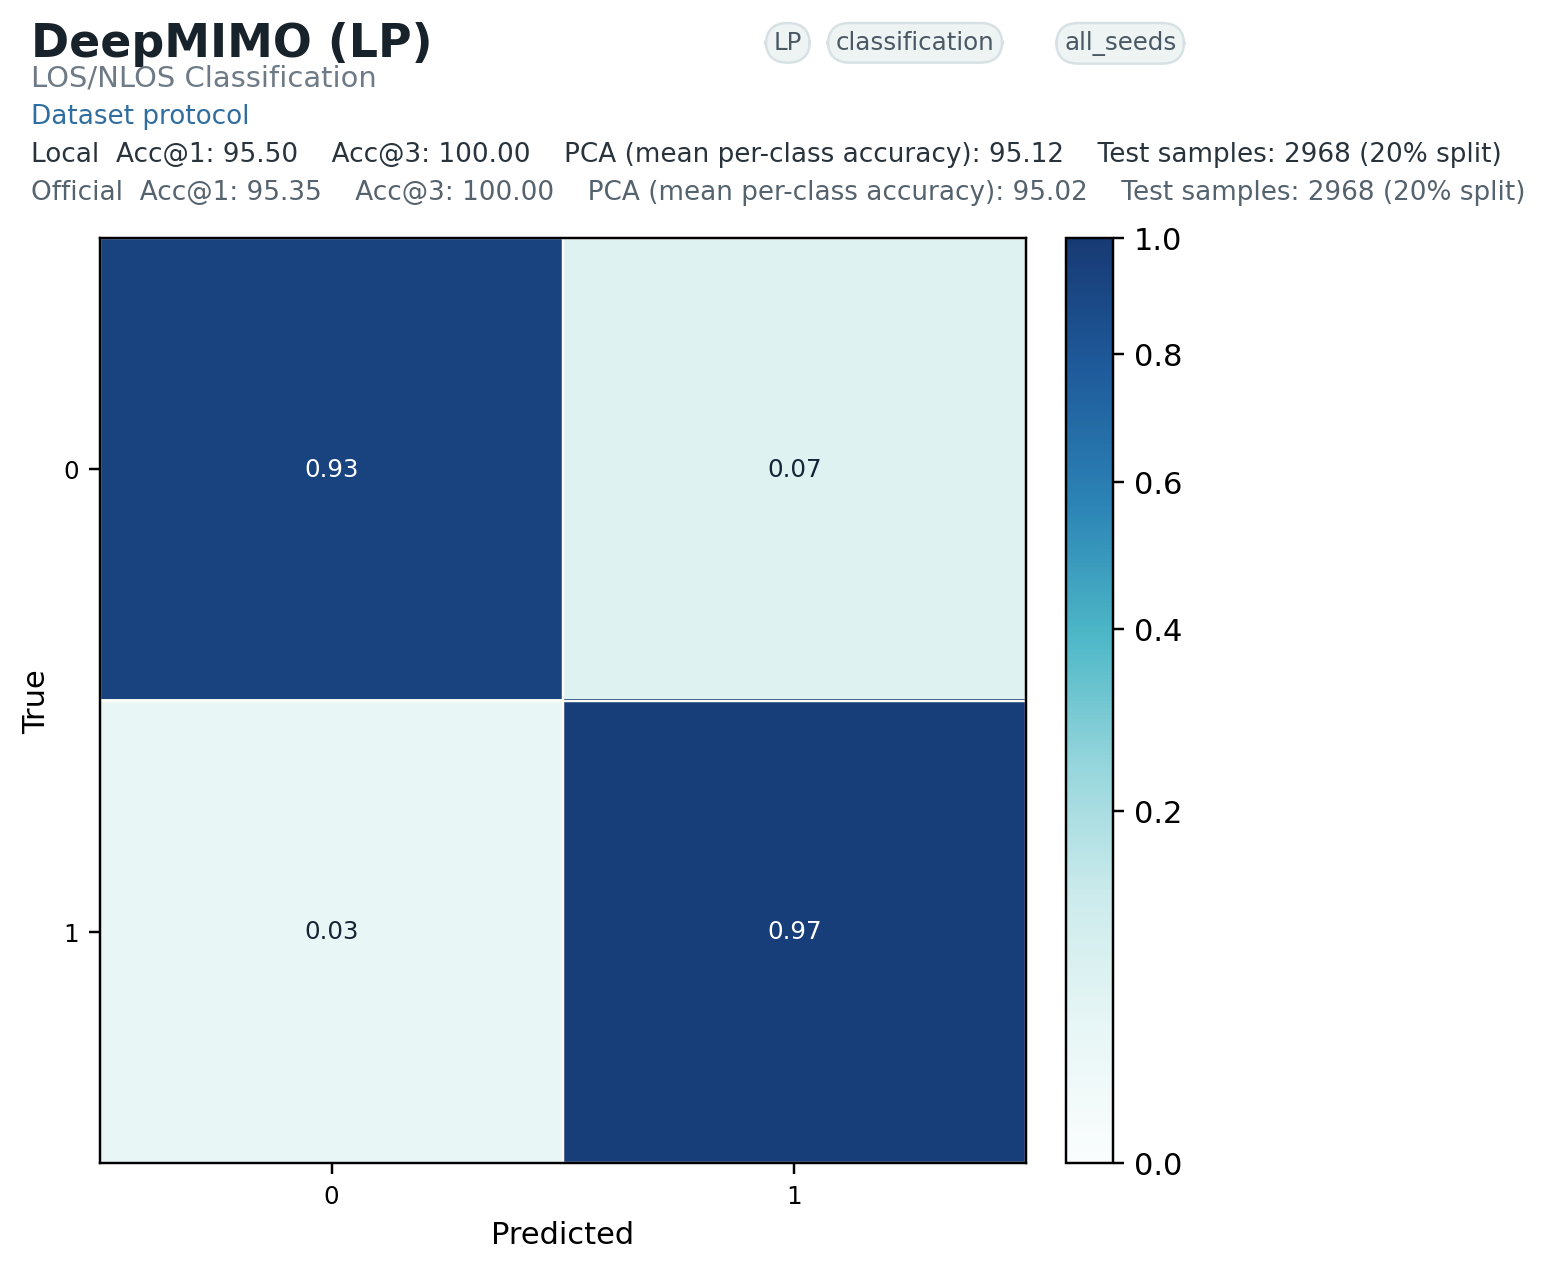
\includegraphics[width=\textwidth]{deepmimo_los_lp_cm.png}
        \caption{LP}
    \end{subfigure}
    \begin{subfigure}[b]{0.48\textwidth}
        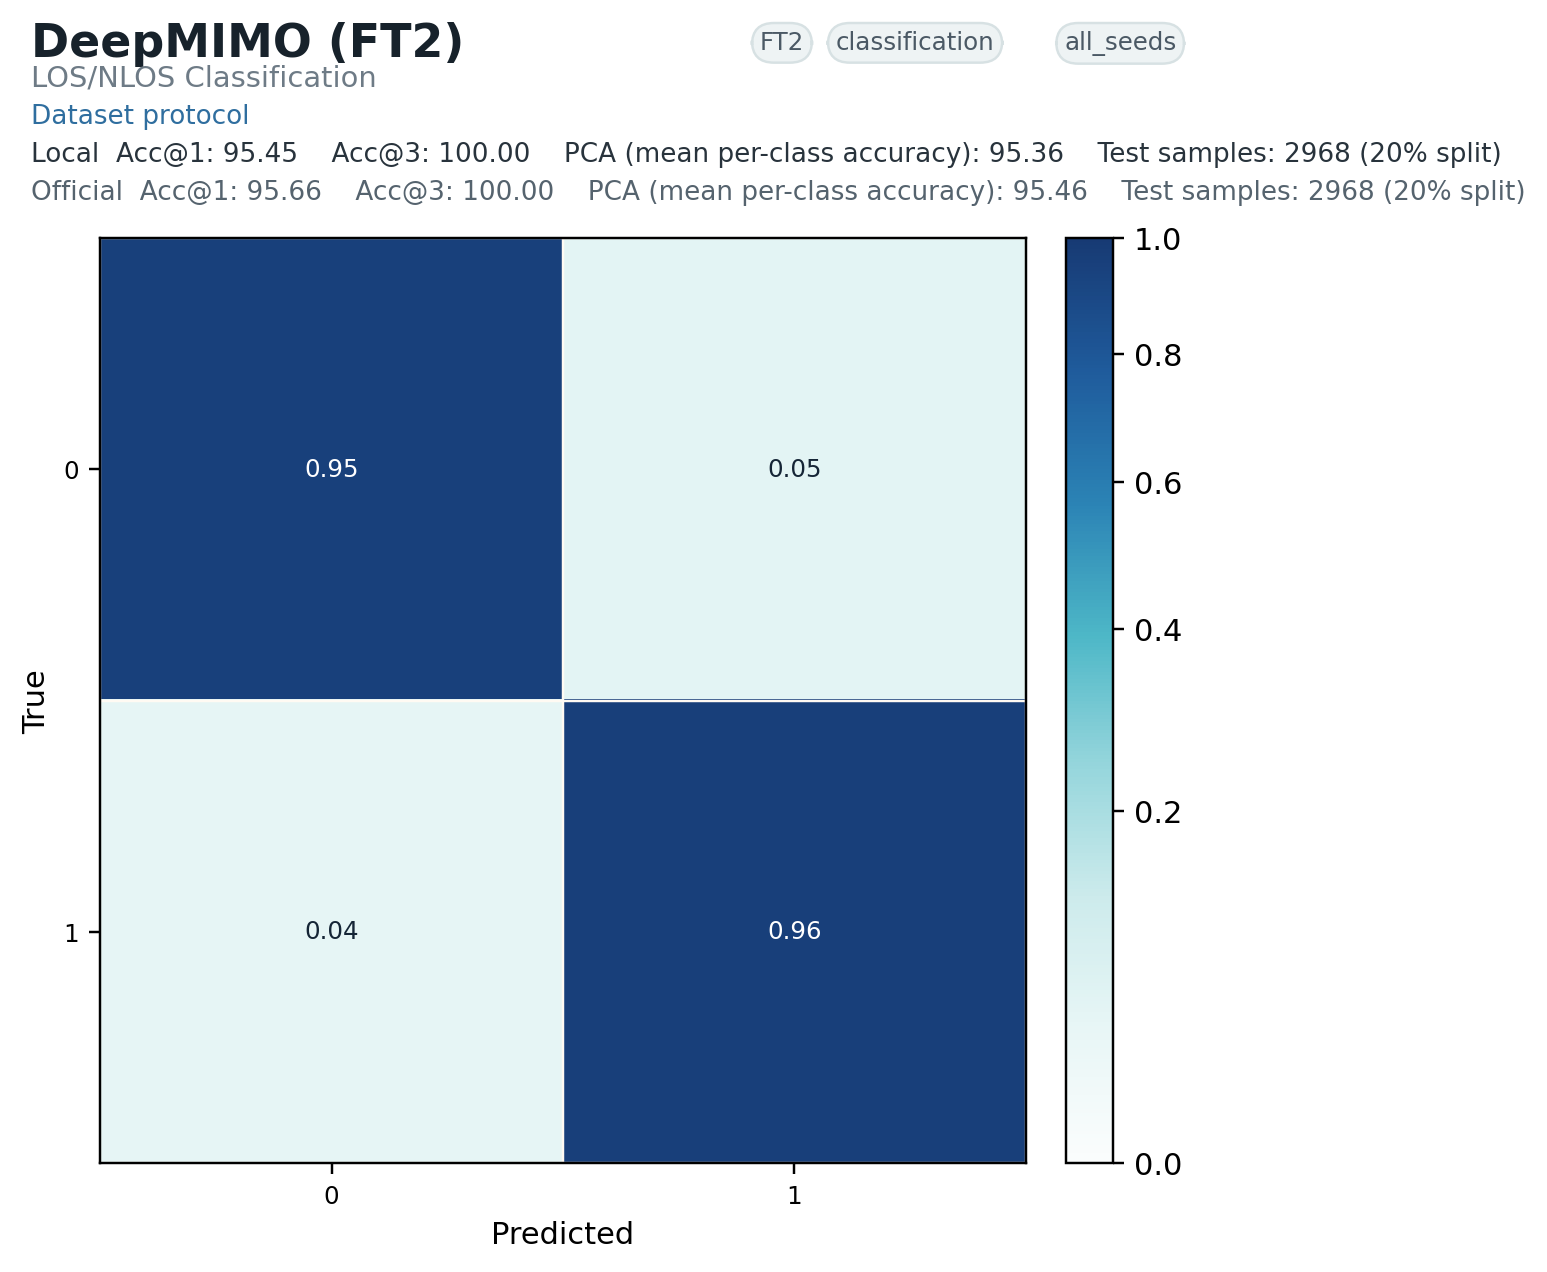
\includegraphics[width=\textwidth]{deepmimo_los_ft2_cm.png}
        \caption{FT2}
    \end{subfigure}
    \begin{subfigure}[b]{0.48\textwidth}
        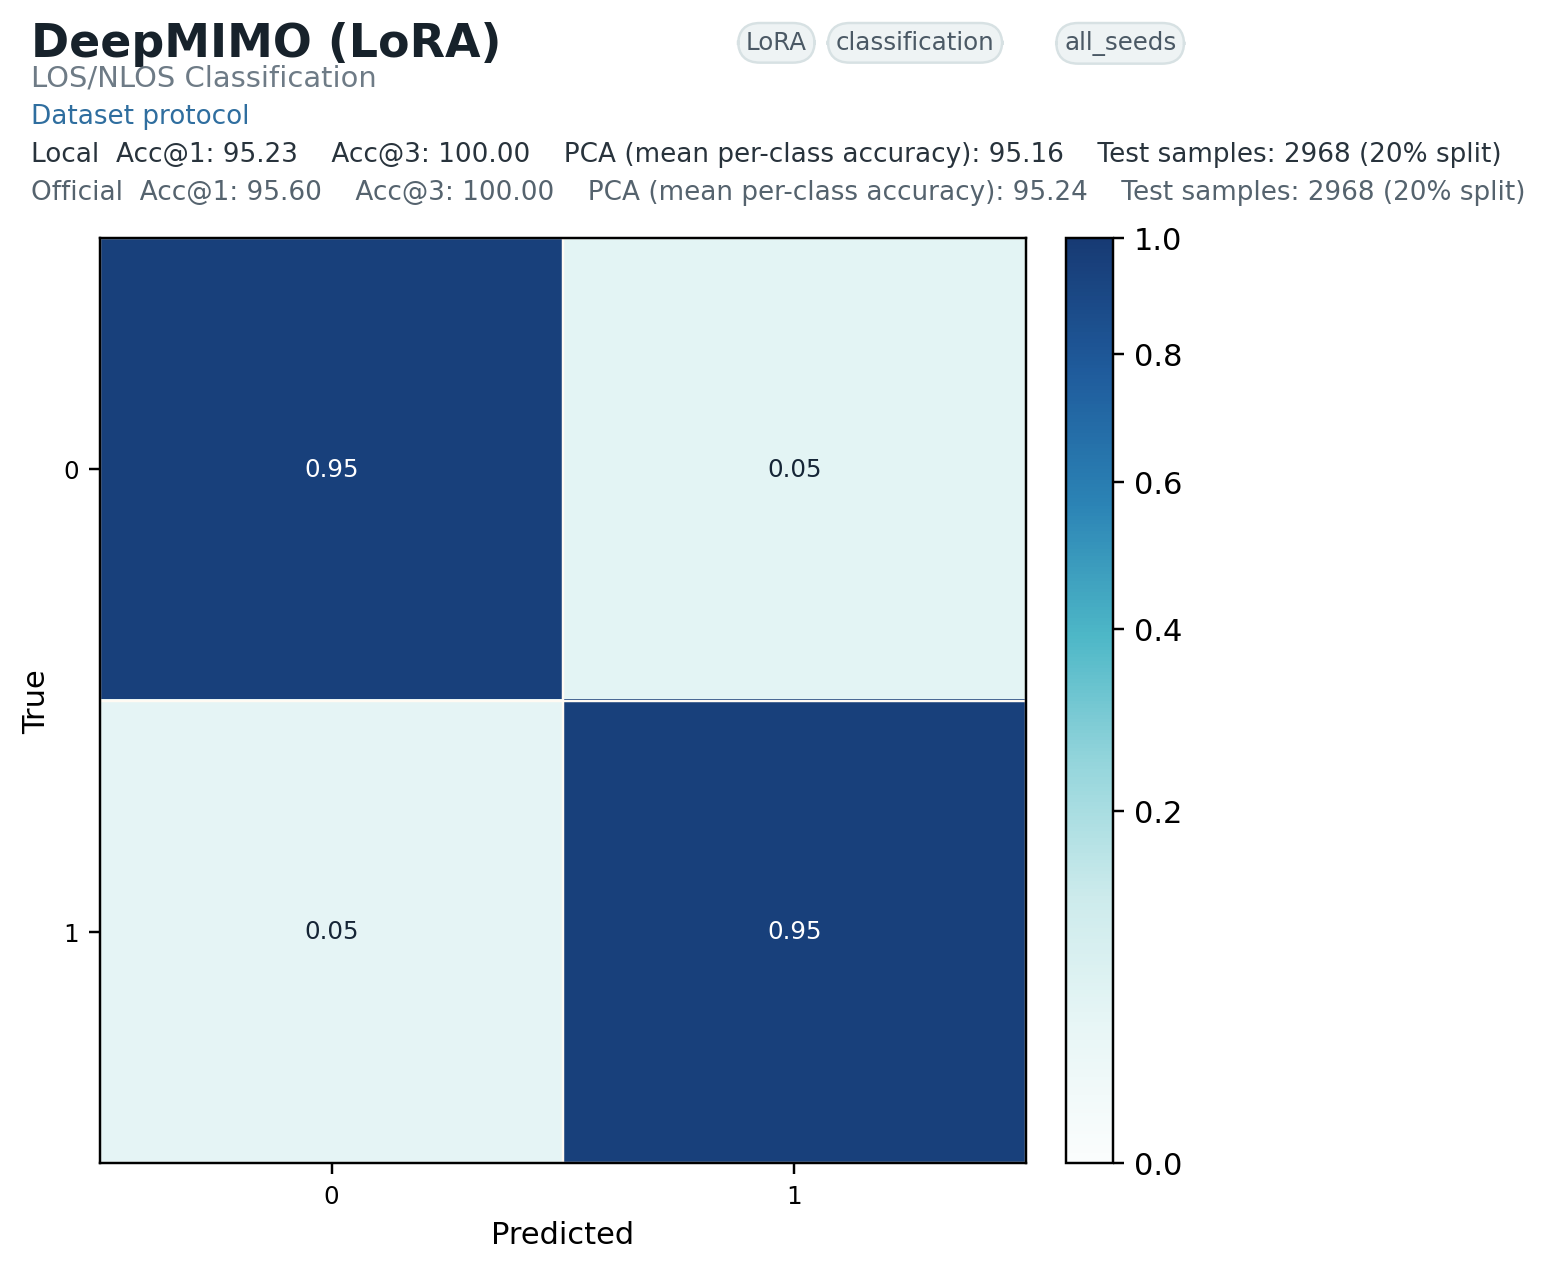
\includegraphics[width=\textwidth]{deepmimo_los_lora_cm.png}
        \caption{LoRA}
    \end{subfigure}
    \caption{Confusion matrices for DeepMIMO LoS/NLoS classification (2 classes). All modes fell within 0.10 percentage points of the official values.}
    \label{fig:deepmimo_los_cm}
\end{figure}

\begin{figure}[H]
    \centering
    \begin{subfigure}[b]{0.48\textwidth}
        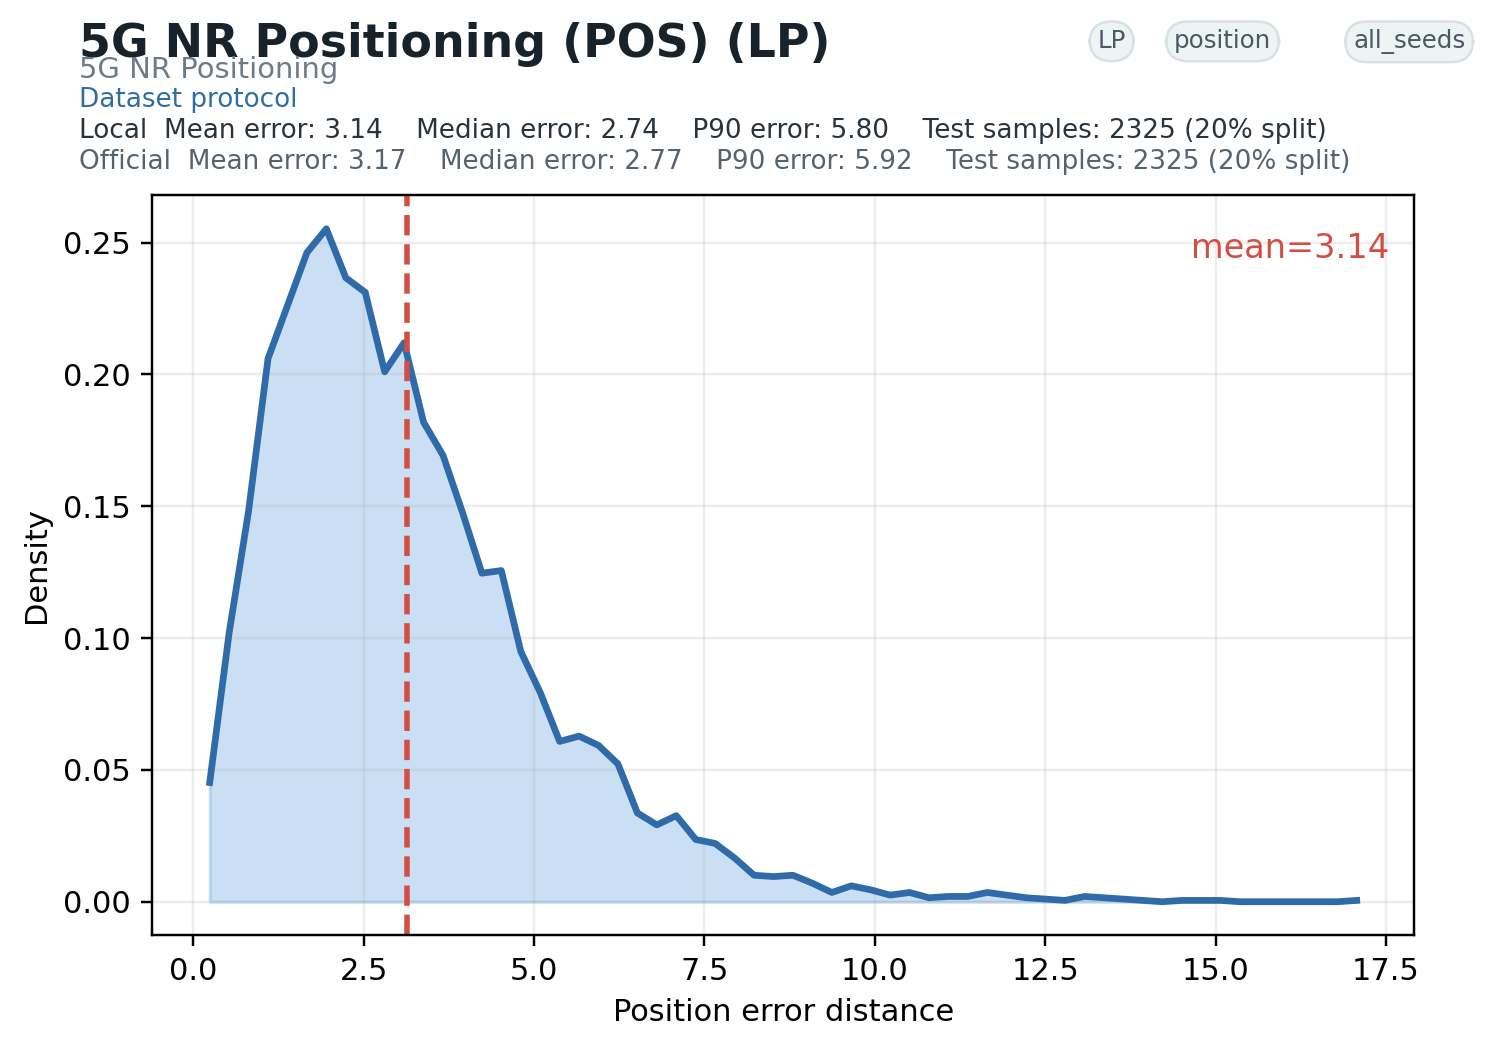
\includegraphics[width=\textwidth]{pos_lp_density.png}
        \caption{POS -- LP}
    \end{subfigure}
    \begin{subfigure}[b]{0.48\textwidth}
        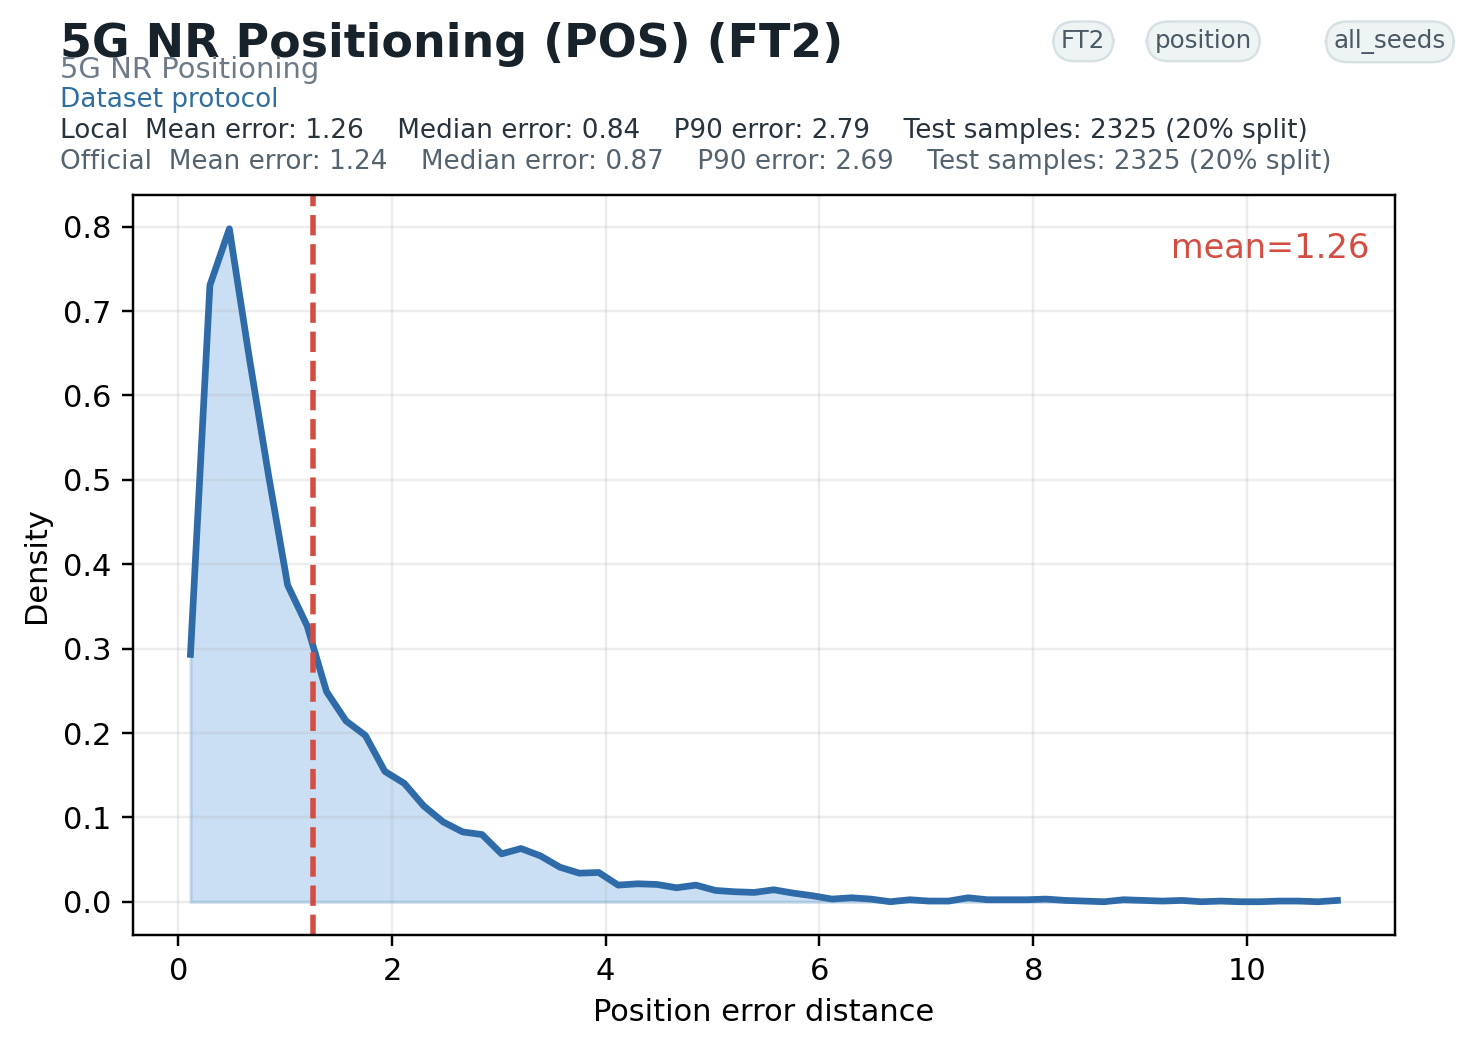
\includegraphics[width=\textwidth]{pos_ft2_density.png}
        \caption{POS -- FT2}
    \end{subfigure}
    \begin{subfigure}[b]{0.48\textwidth}
        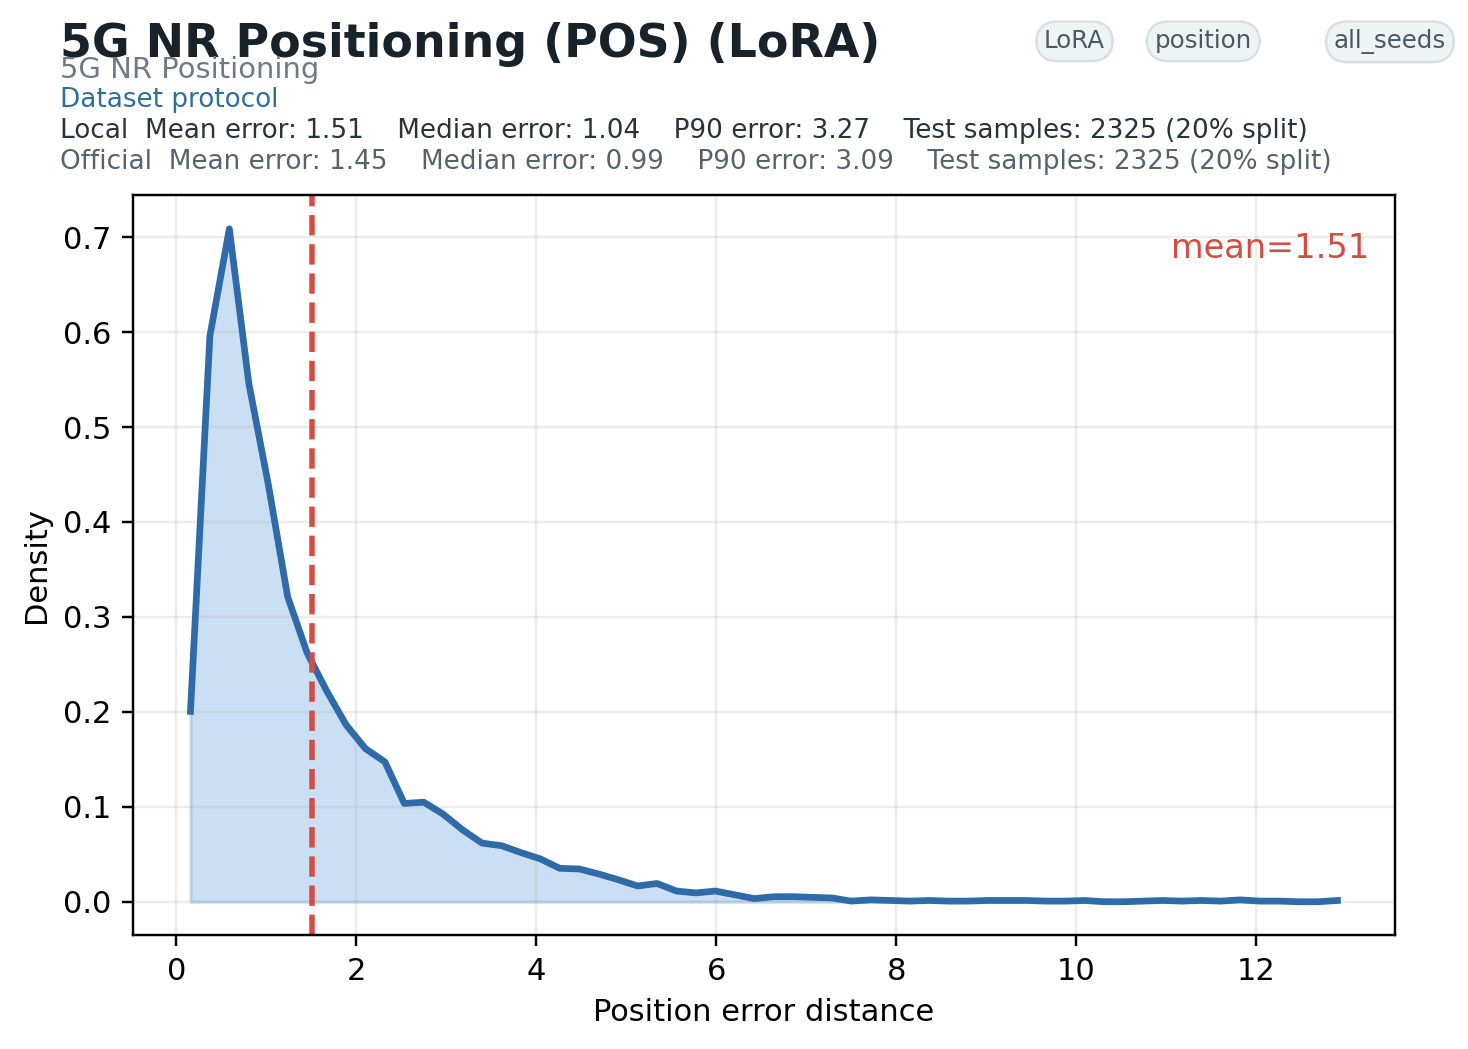
\includegraphics[width=\textwidth]{pos_lora_density.png}
        \caption{POS -- LoRA}
    \end{subfigure}
    \caption{Position error density for 5G NR Positioning. A curve concentrated near zero indicates accurate localization. The shift from LP to FT2/LoRA shows clear improvement.}
    \label{fig:pos_density}
\end{figure}

\begin{figure}[H]
    \centering
    \begin{subfigure}[b]{0.48\textwidth}
        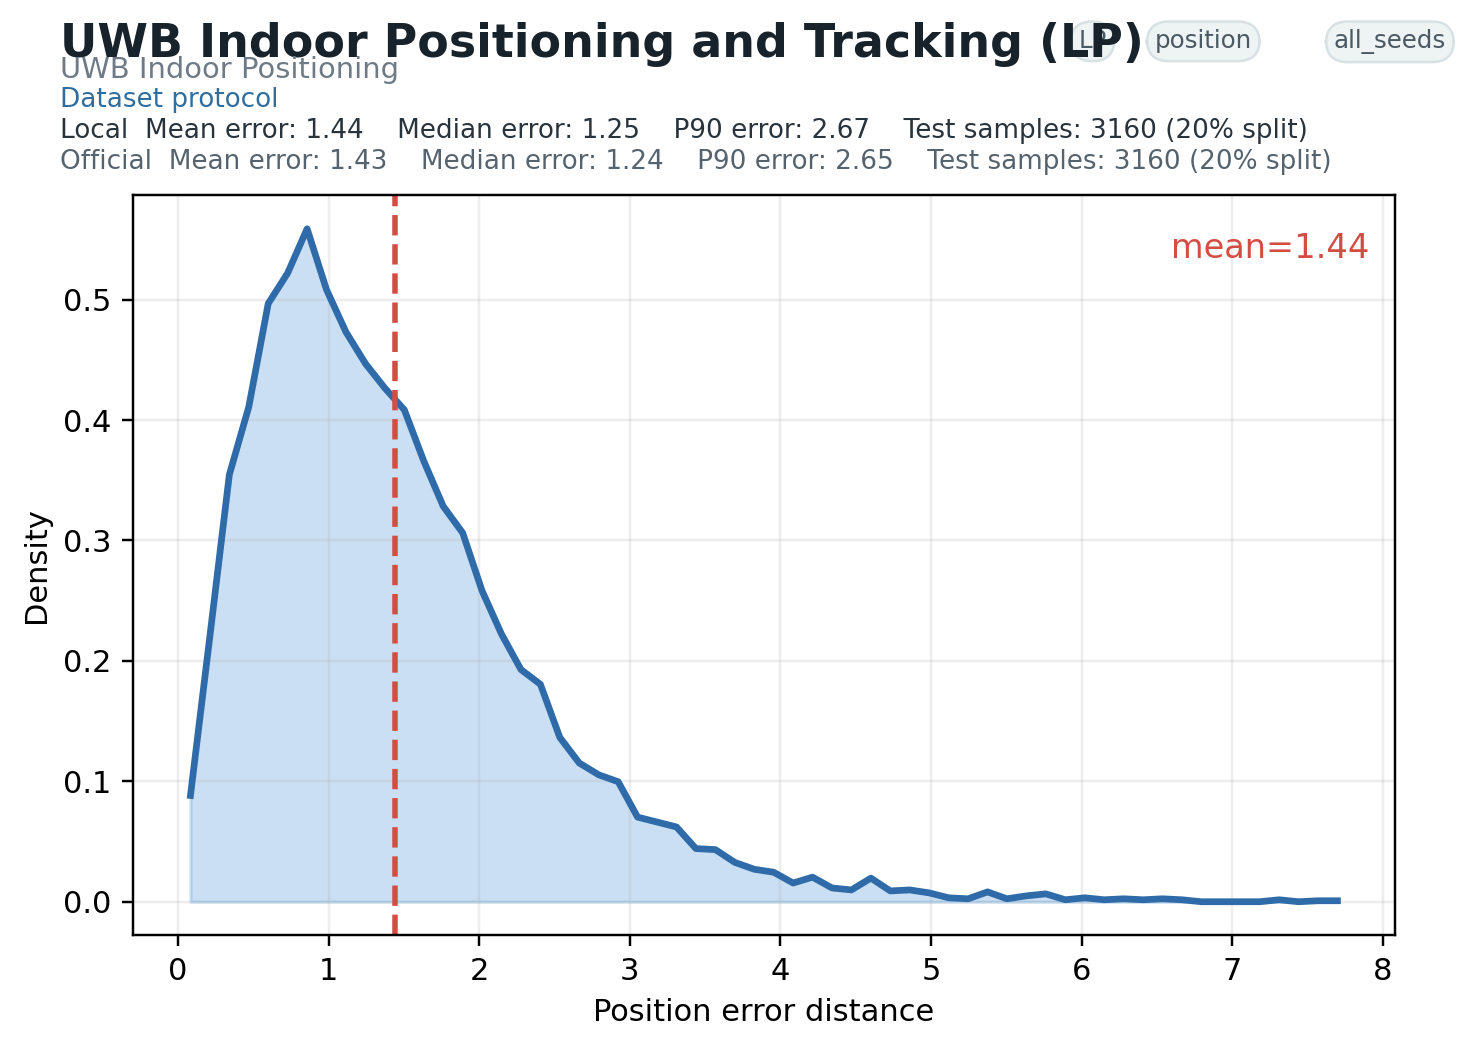
\includegraphics[width=\textwidth]{uwb_indoor_lp_density.png}
        \caption{UWB Indoor -- LP}
    \end{subfigure}
    \begin{subfigure}[b]{0.48\textwidth}
        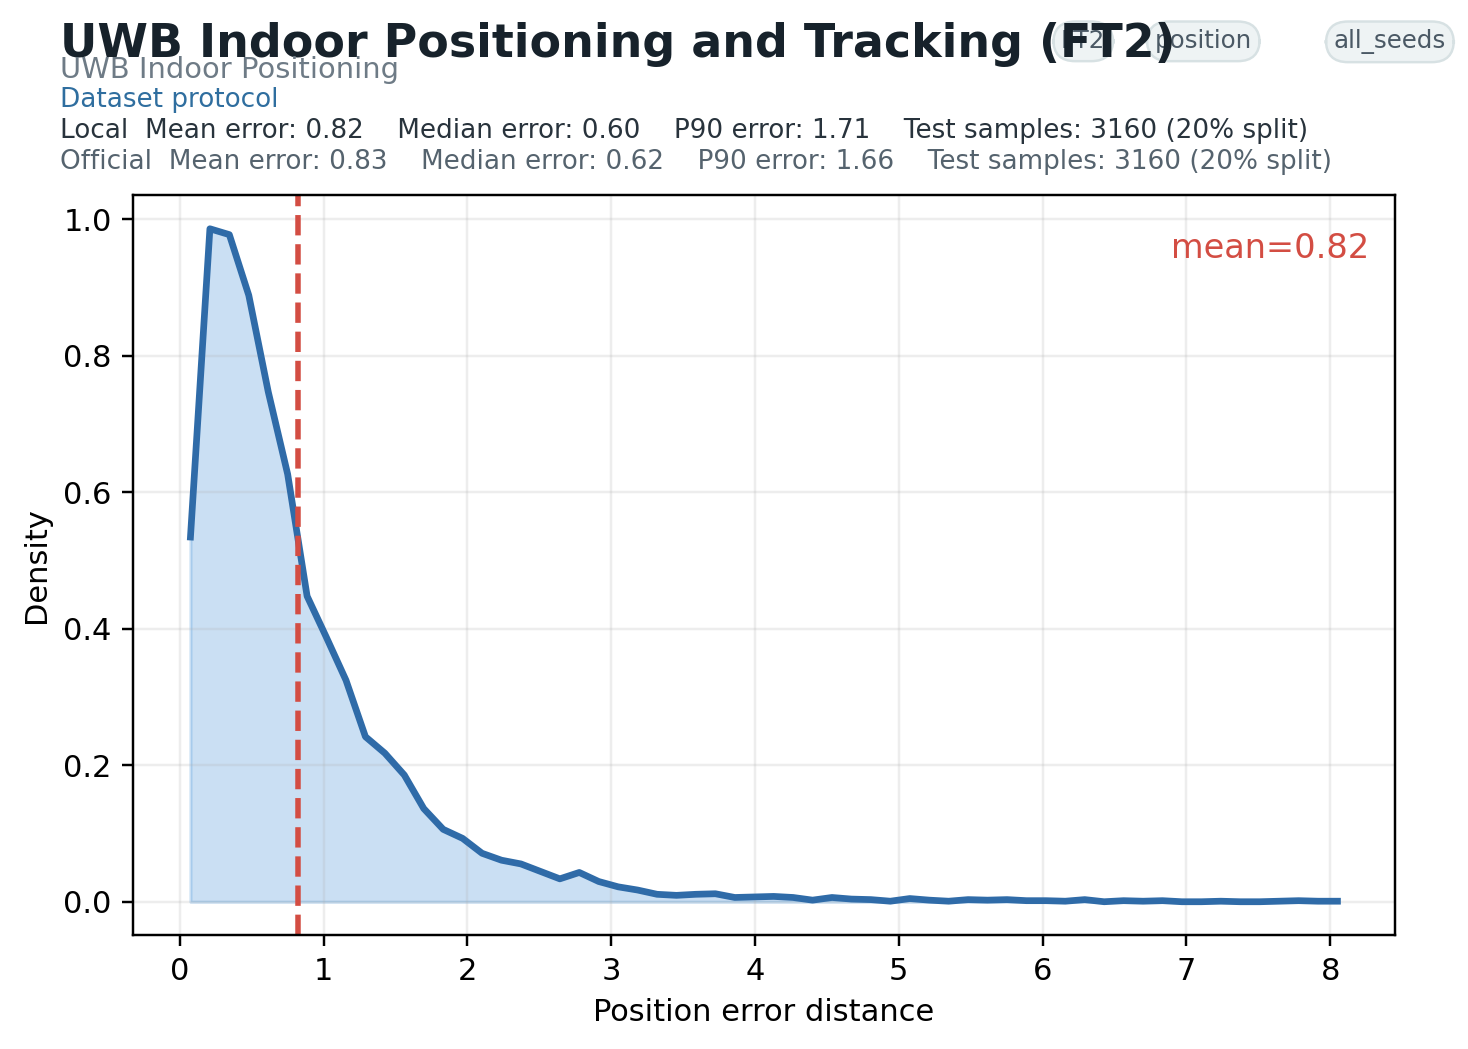
\includegraphics[width=\textwidth]{uwb_indoor_ft2_density.png}
        \caption{UWB Indoor -- FT2}
    \end{subfigure}
    \begin{subfigure}[b]{0.48\textwidth}
        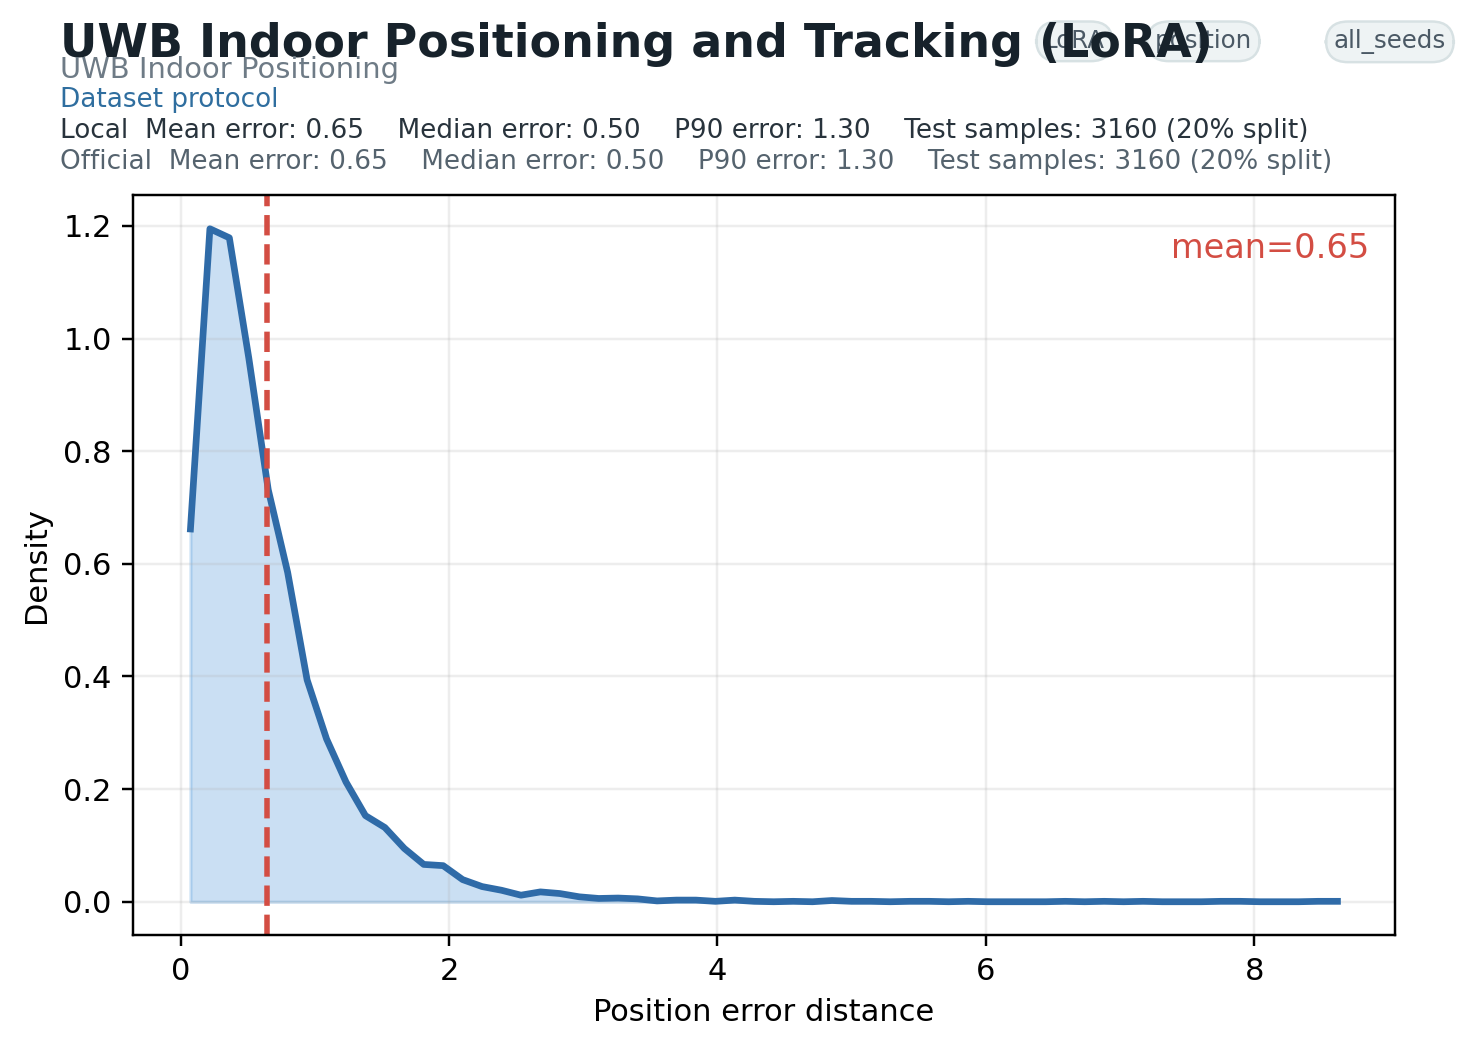
\includegraphics[width=\textwidth]{uwb_indoor_lora_density.png}
        \caption{UWB Indoor -- LoRA}
    \end{subfigure}
    \caption{Position error density for UWB Indoor localization.}
    \label{fig:uwb_indoor_density}
\end{figure}

\begin{figure}[H]
    \centering
    \begin{subfigure}[b]{0.48\textwidth}
        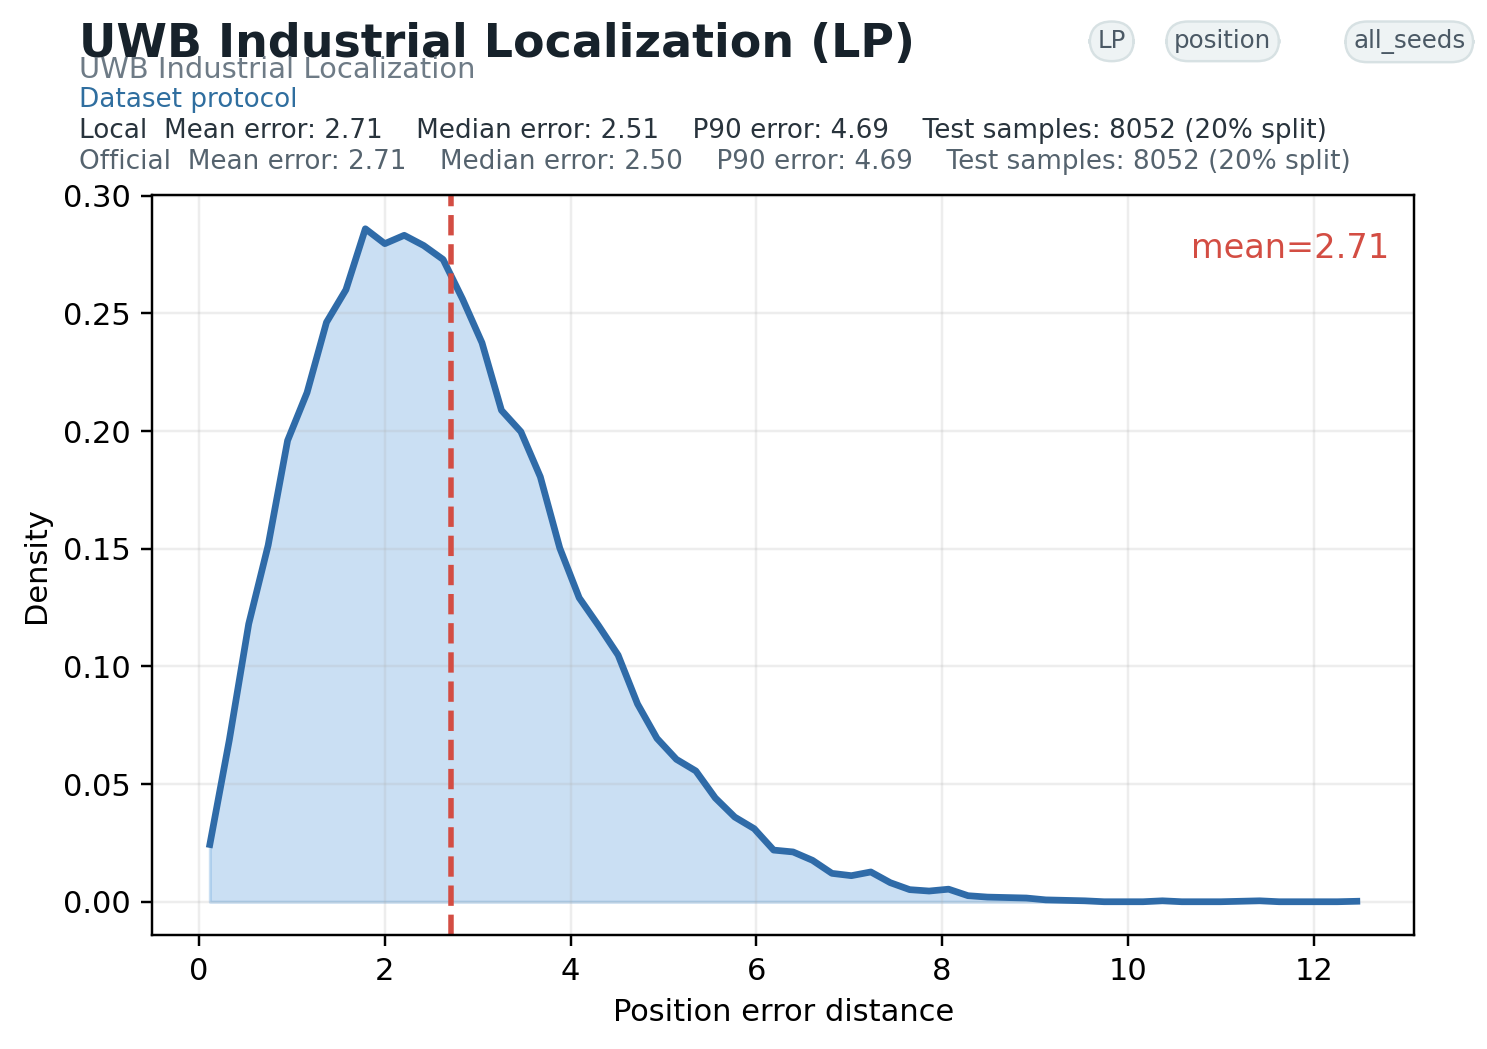
\includegraphics[width=\textwidth]{uwb_industrial_lp_density.png}
        \caption{UWB Industrial -- LP}
    \end{subfigure}
    \begin{subfigure}[b]{0.48\textwidth}
        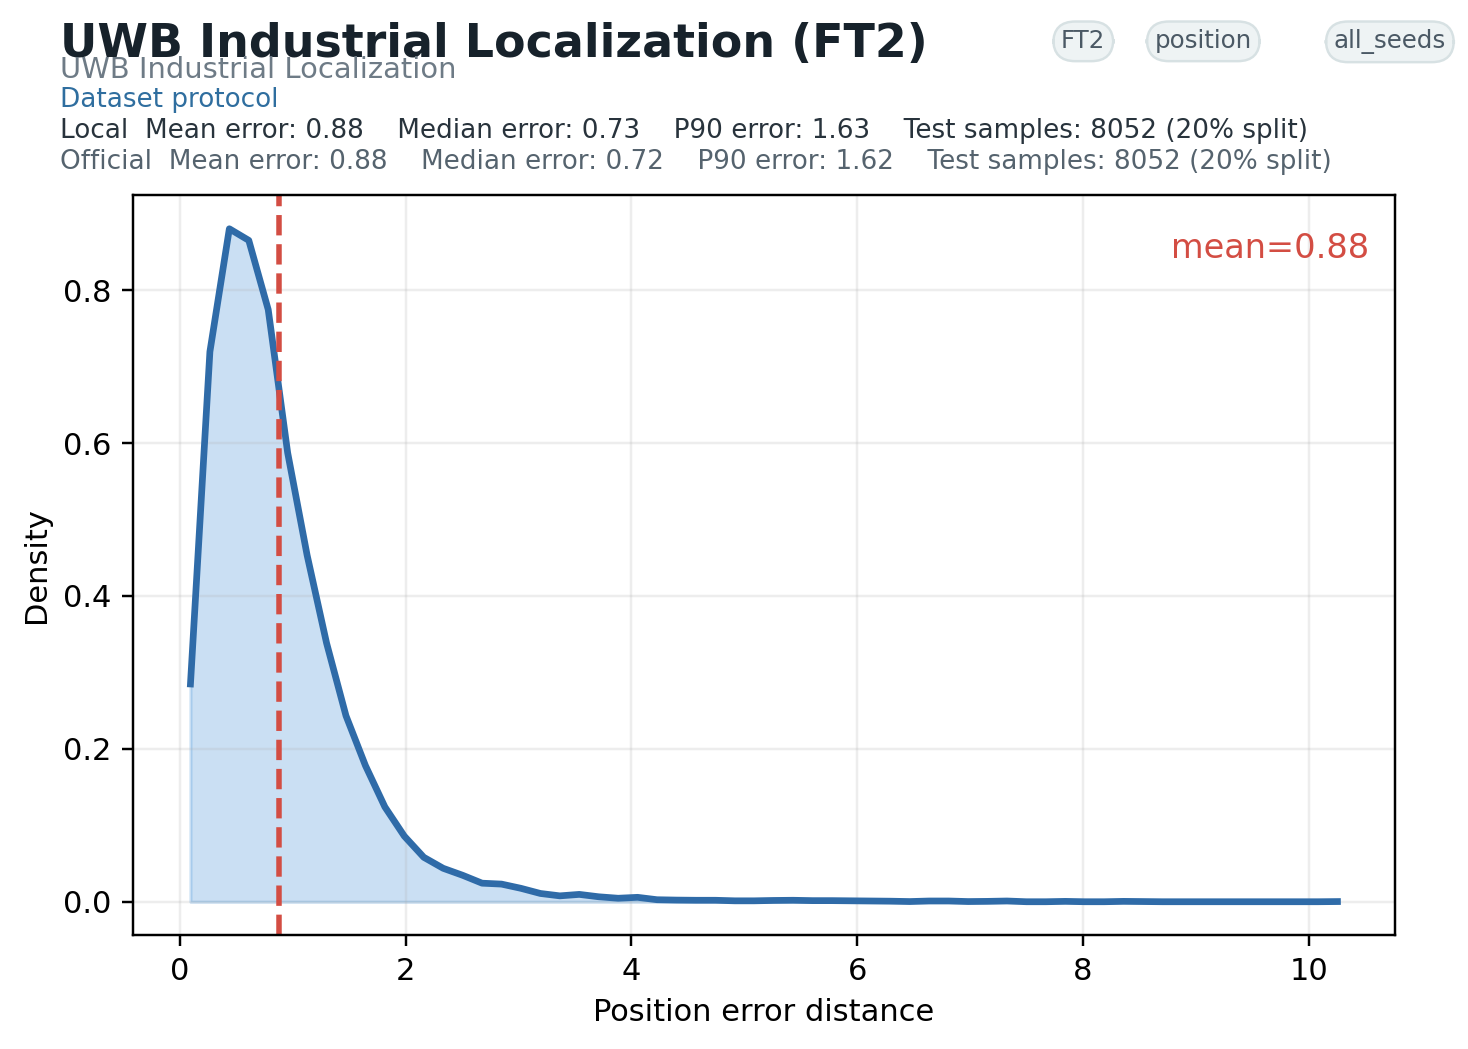
\includegraphics[width=\textwidth]{uwb_industrial_ft2_density.png}
        \caption{UWB Industrial -- FT2}
    \end{subfigure}
    \begin{subfigure}[b]{0.48\textwidth}
        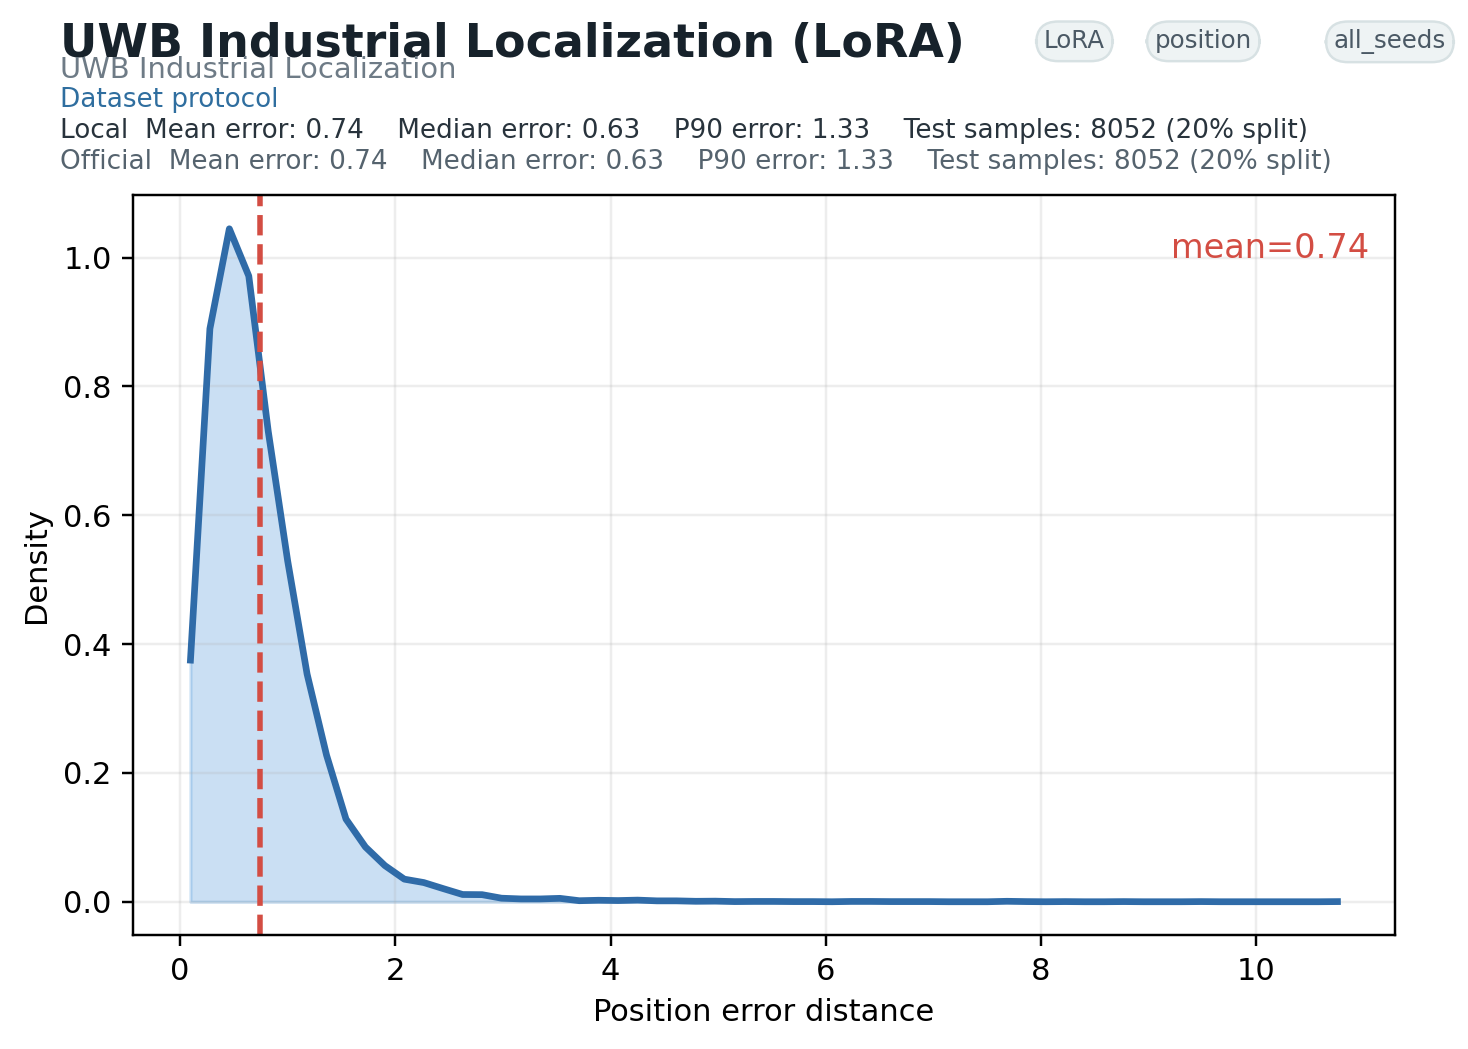
\includegraphics[width=\textwidth]{uwb_industrial_lora_density.png}
        \caption{UWB Industrial -- LoRA}
    \end{subfigure}
    \caption{Position error density for UWB Industrial localization.}
    \label{fig:uwb_industrial_density}
\end{figure}

\begin{figure}[H]
    \centering
    \begin{subfigure}[b]{0.48\textwidth}
        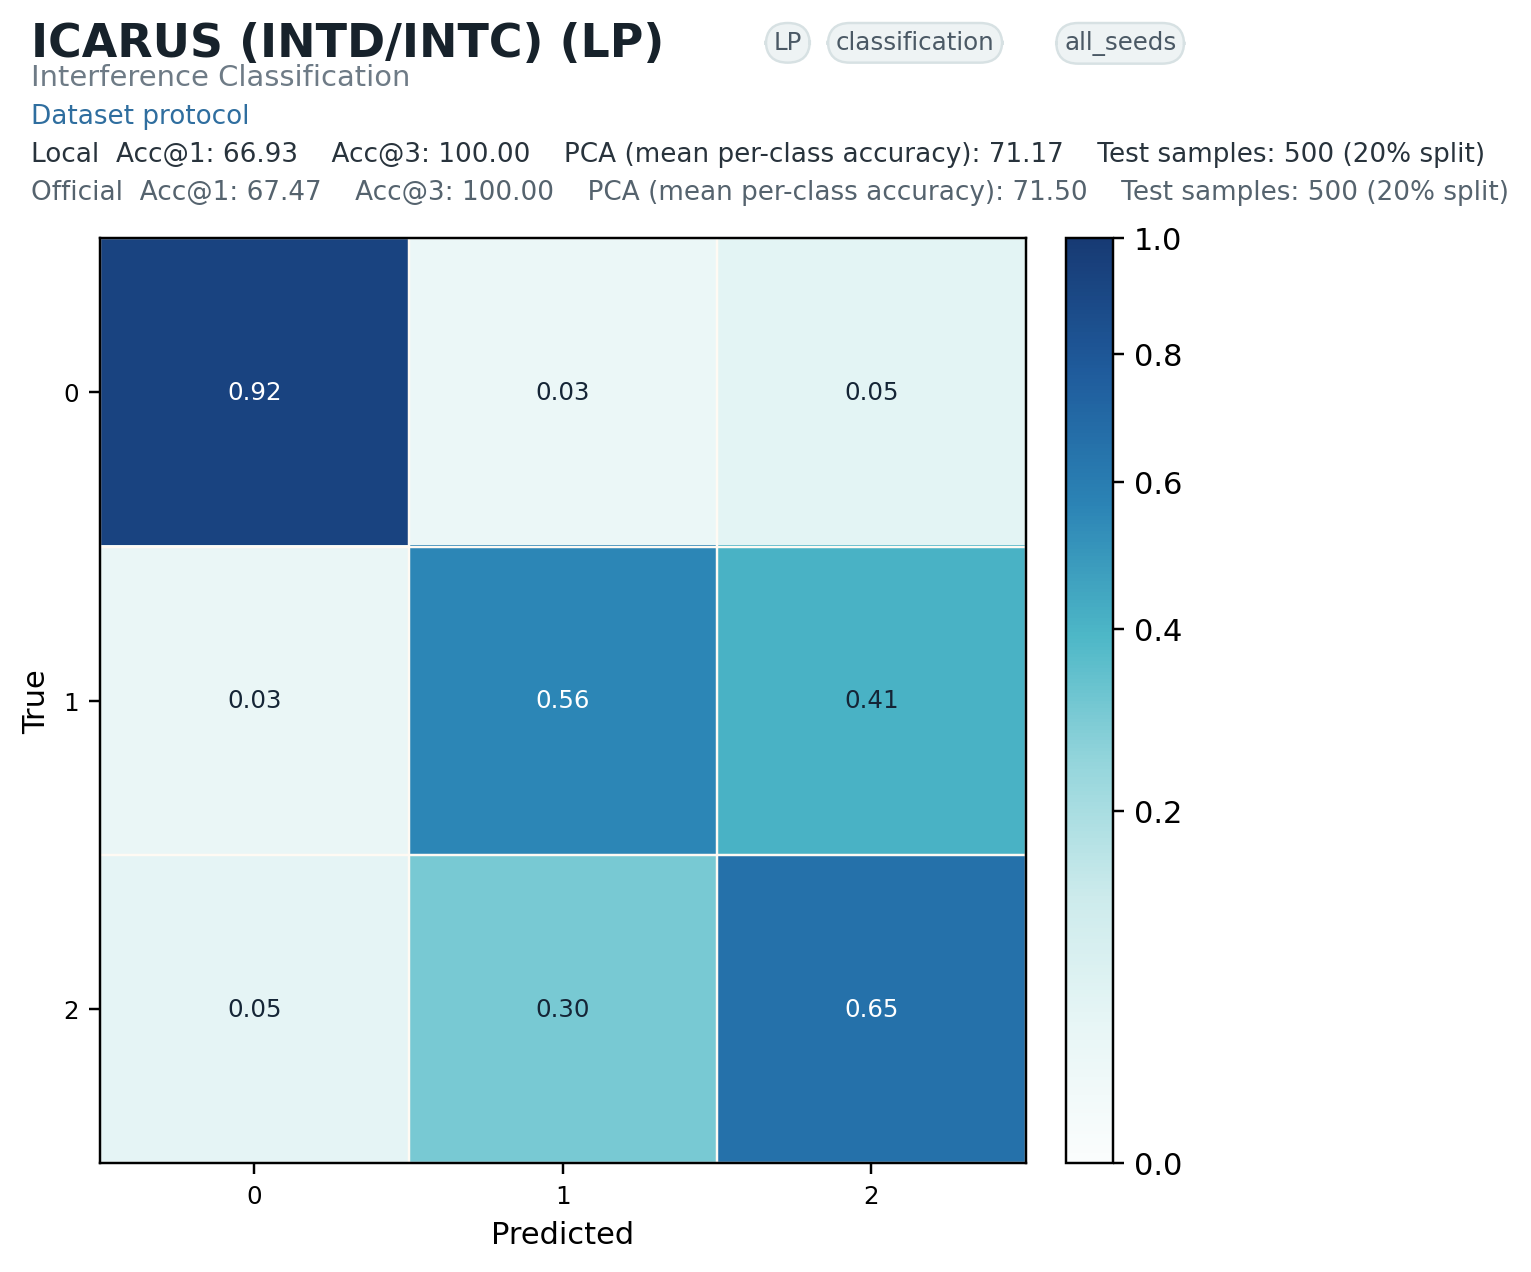
\includegraphics[width=\textwidth]{interf_lp_cm.png}
        \caption{Interference -- LP}
    \end{subfigure}
    \begin{subfigure}[b]{0.48\textwidth}
        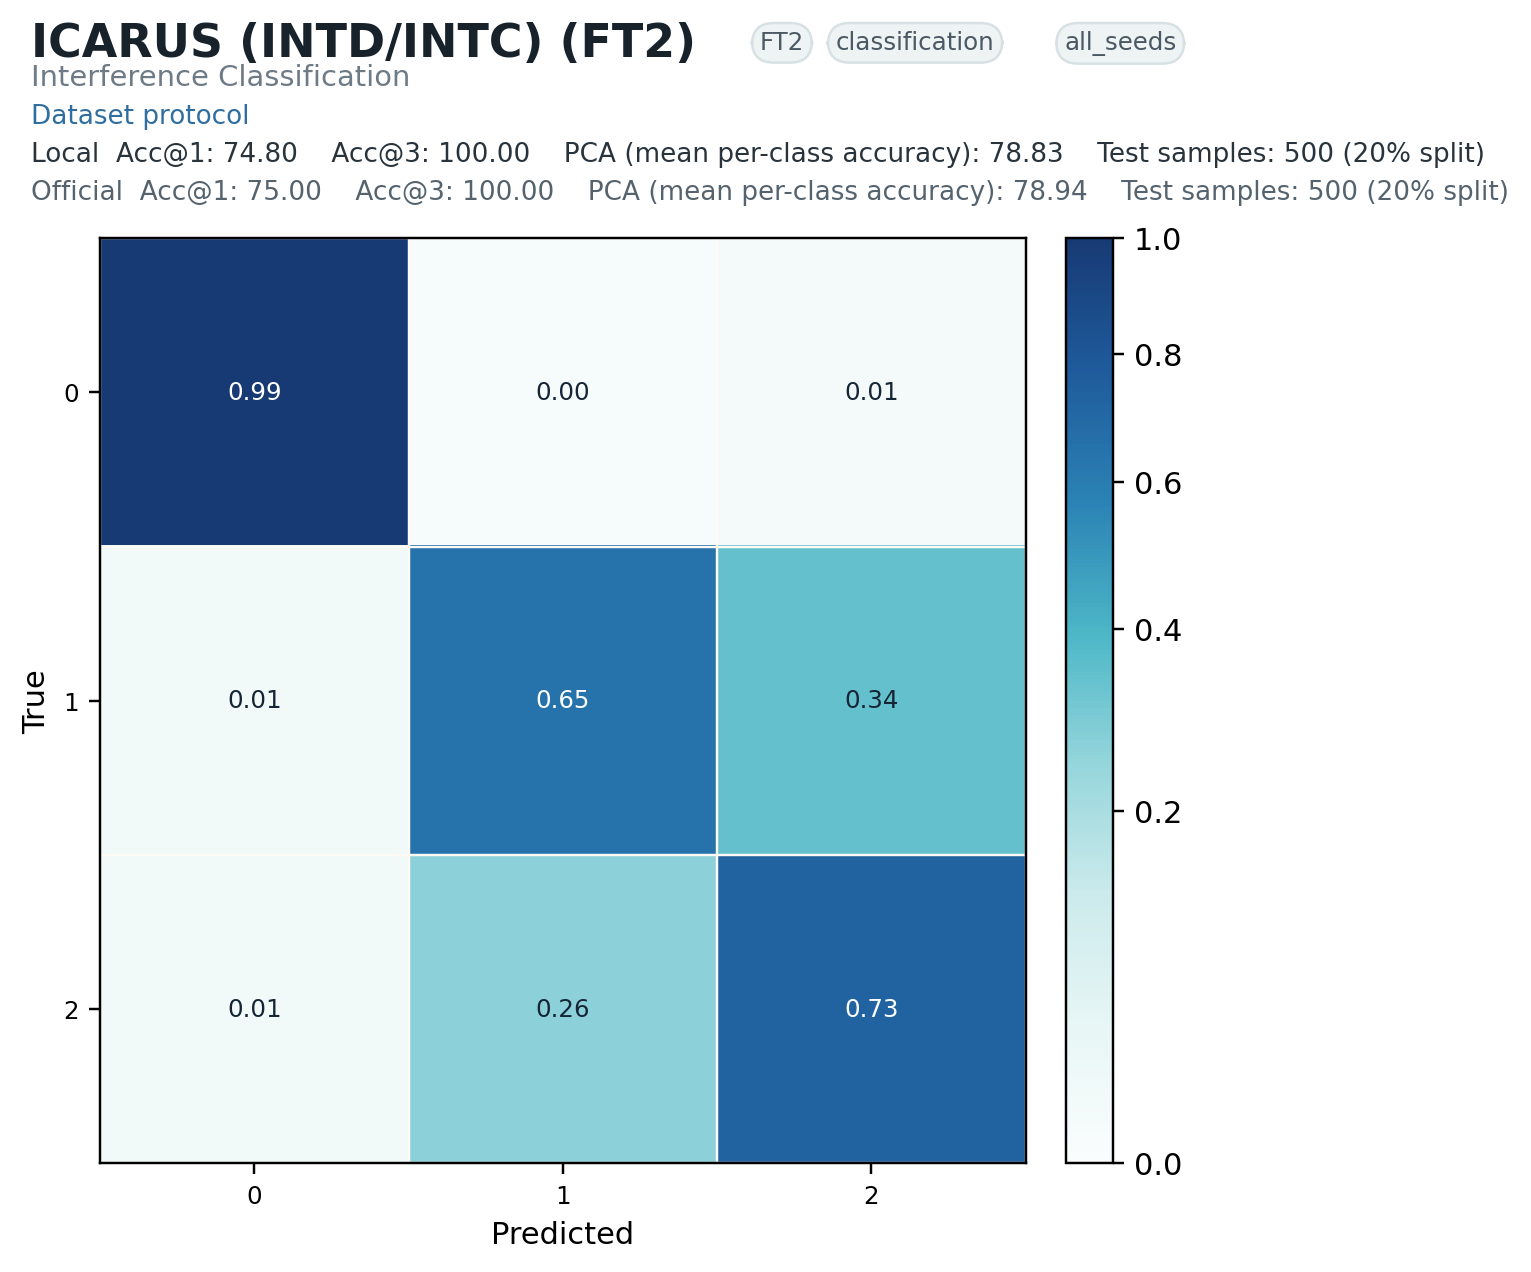
\includegraphics[width=\textwidth]{interf_ft2_cm.png}
        \caption{Interference -- FT2}
    \end{subfigure}
    \begin{subfigure}[b]{0.48\textwidth}
        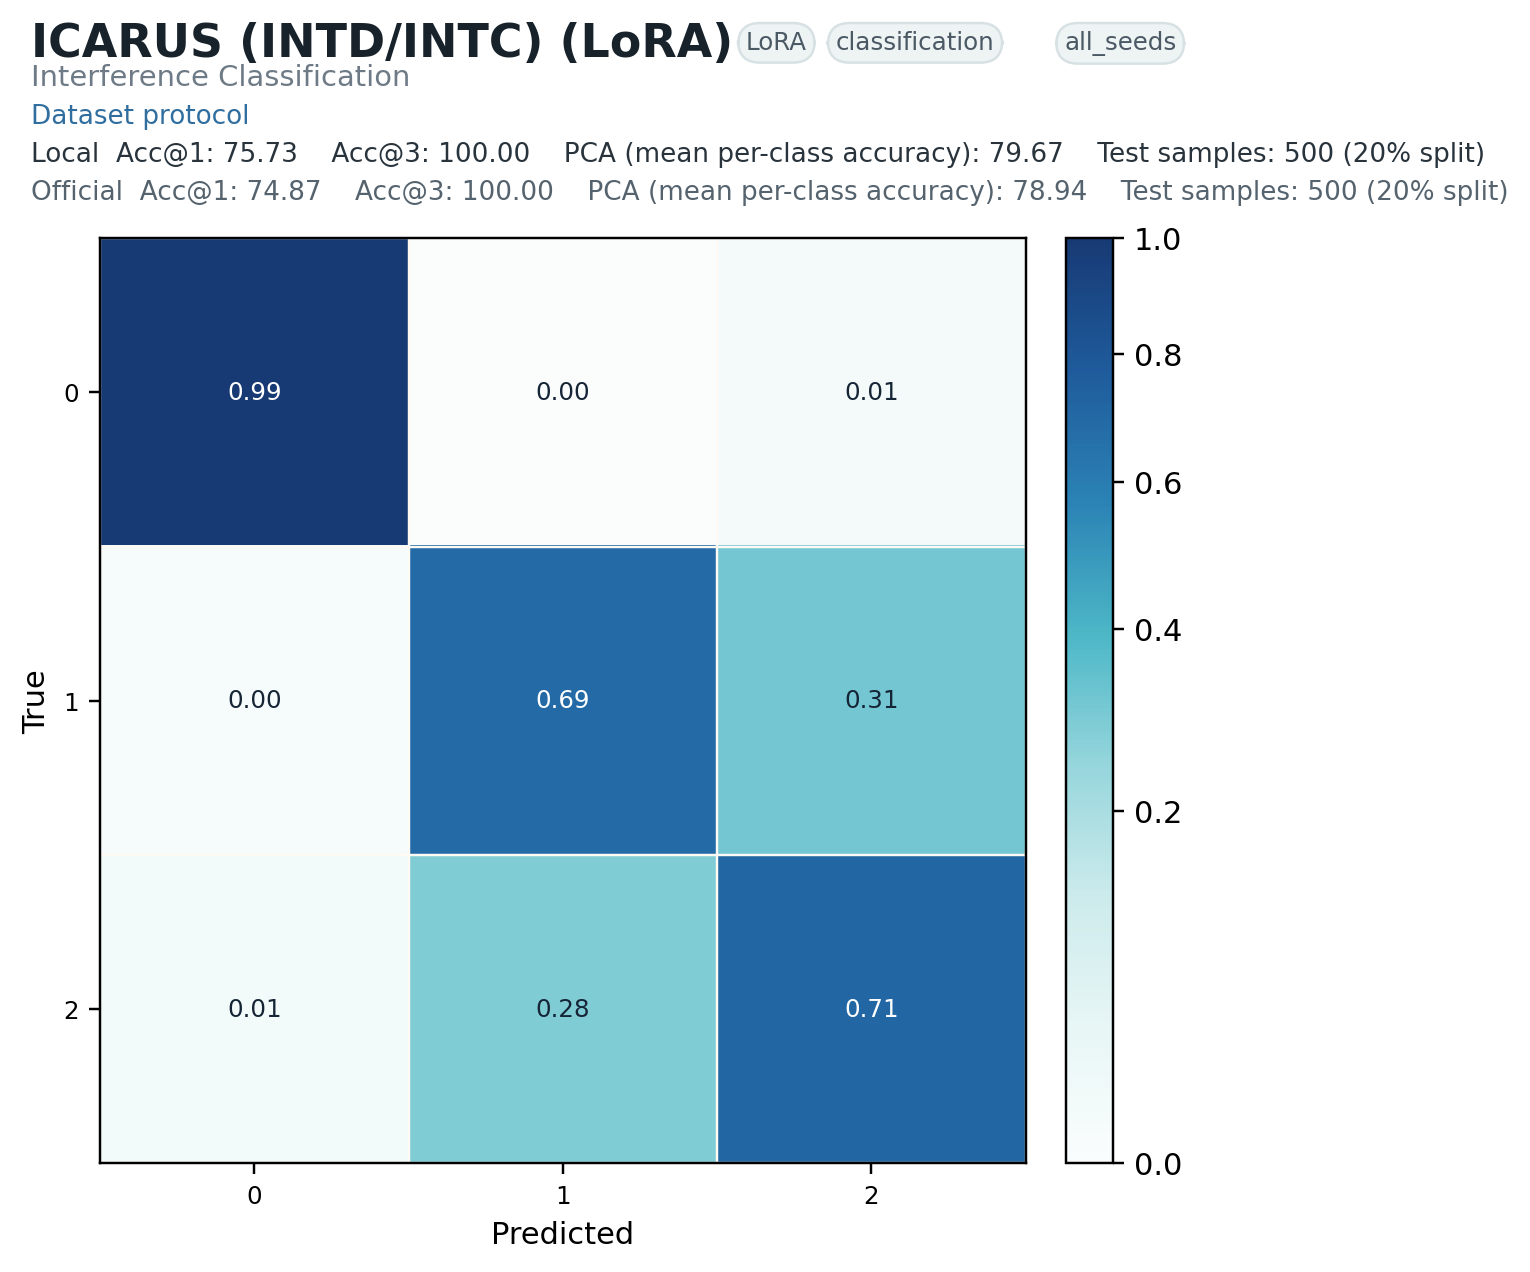
\includegraphics[width=\textwidth]{interf_lora_cm.png}
        \caption{Interference -- LoRA}
    \end{subfigure}
    \caption{Confusion matrices for ICARUS interference classification (3 classes).}
    \label{fig:interf_cm}
\end{figure}

\begin{figure}[H]
    \centering
    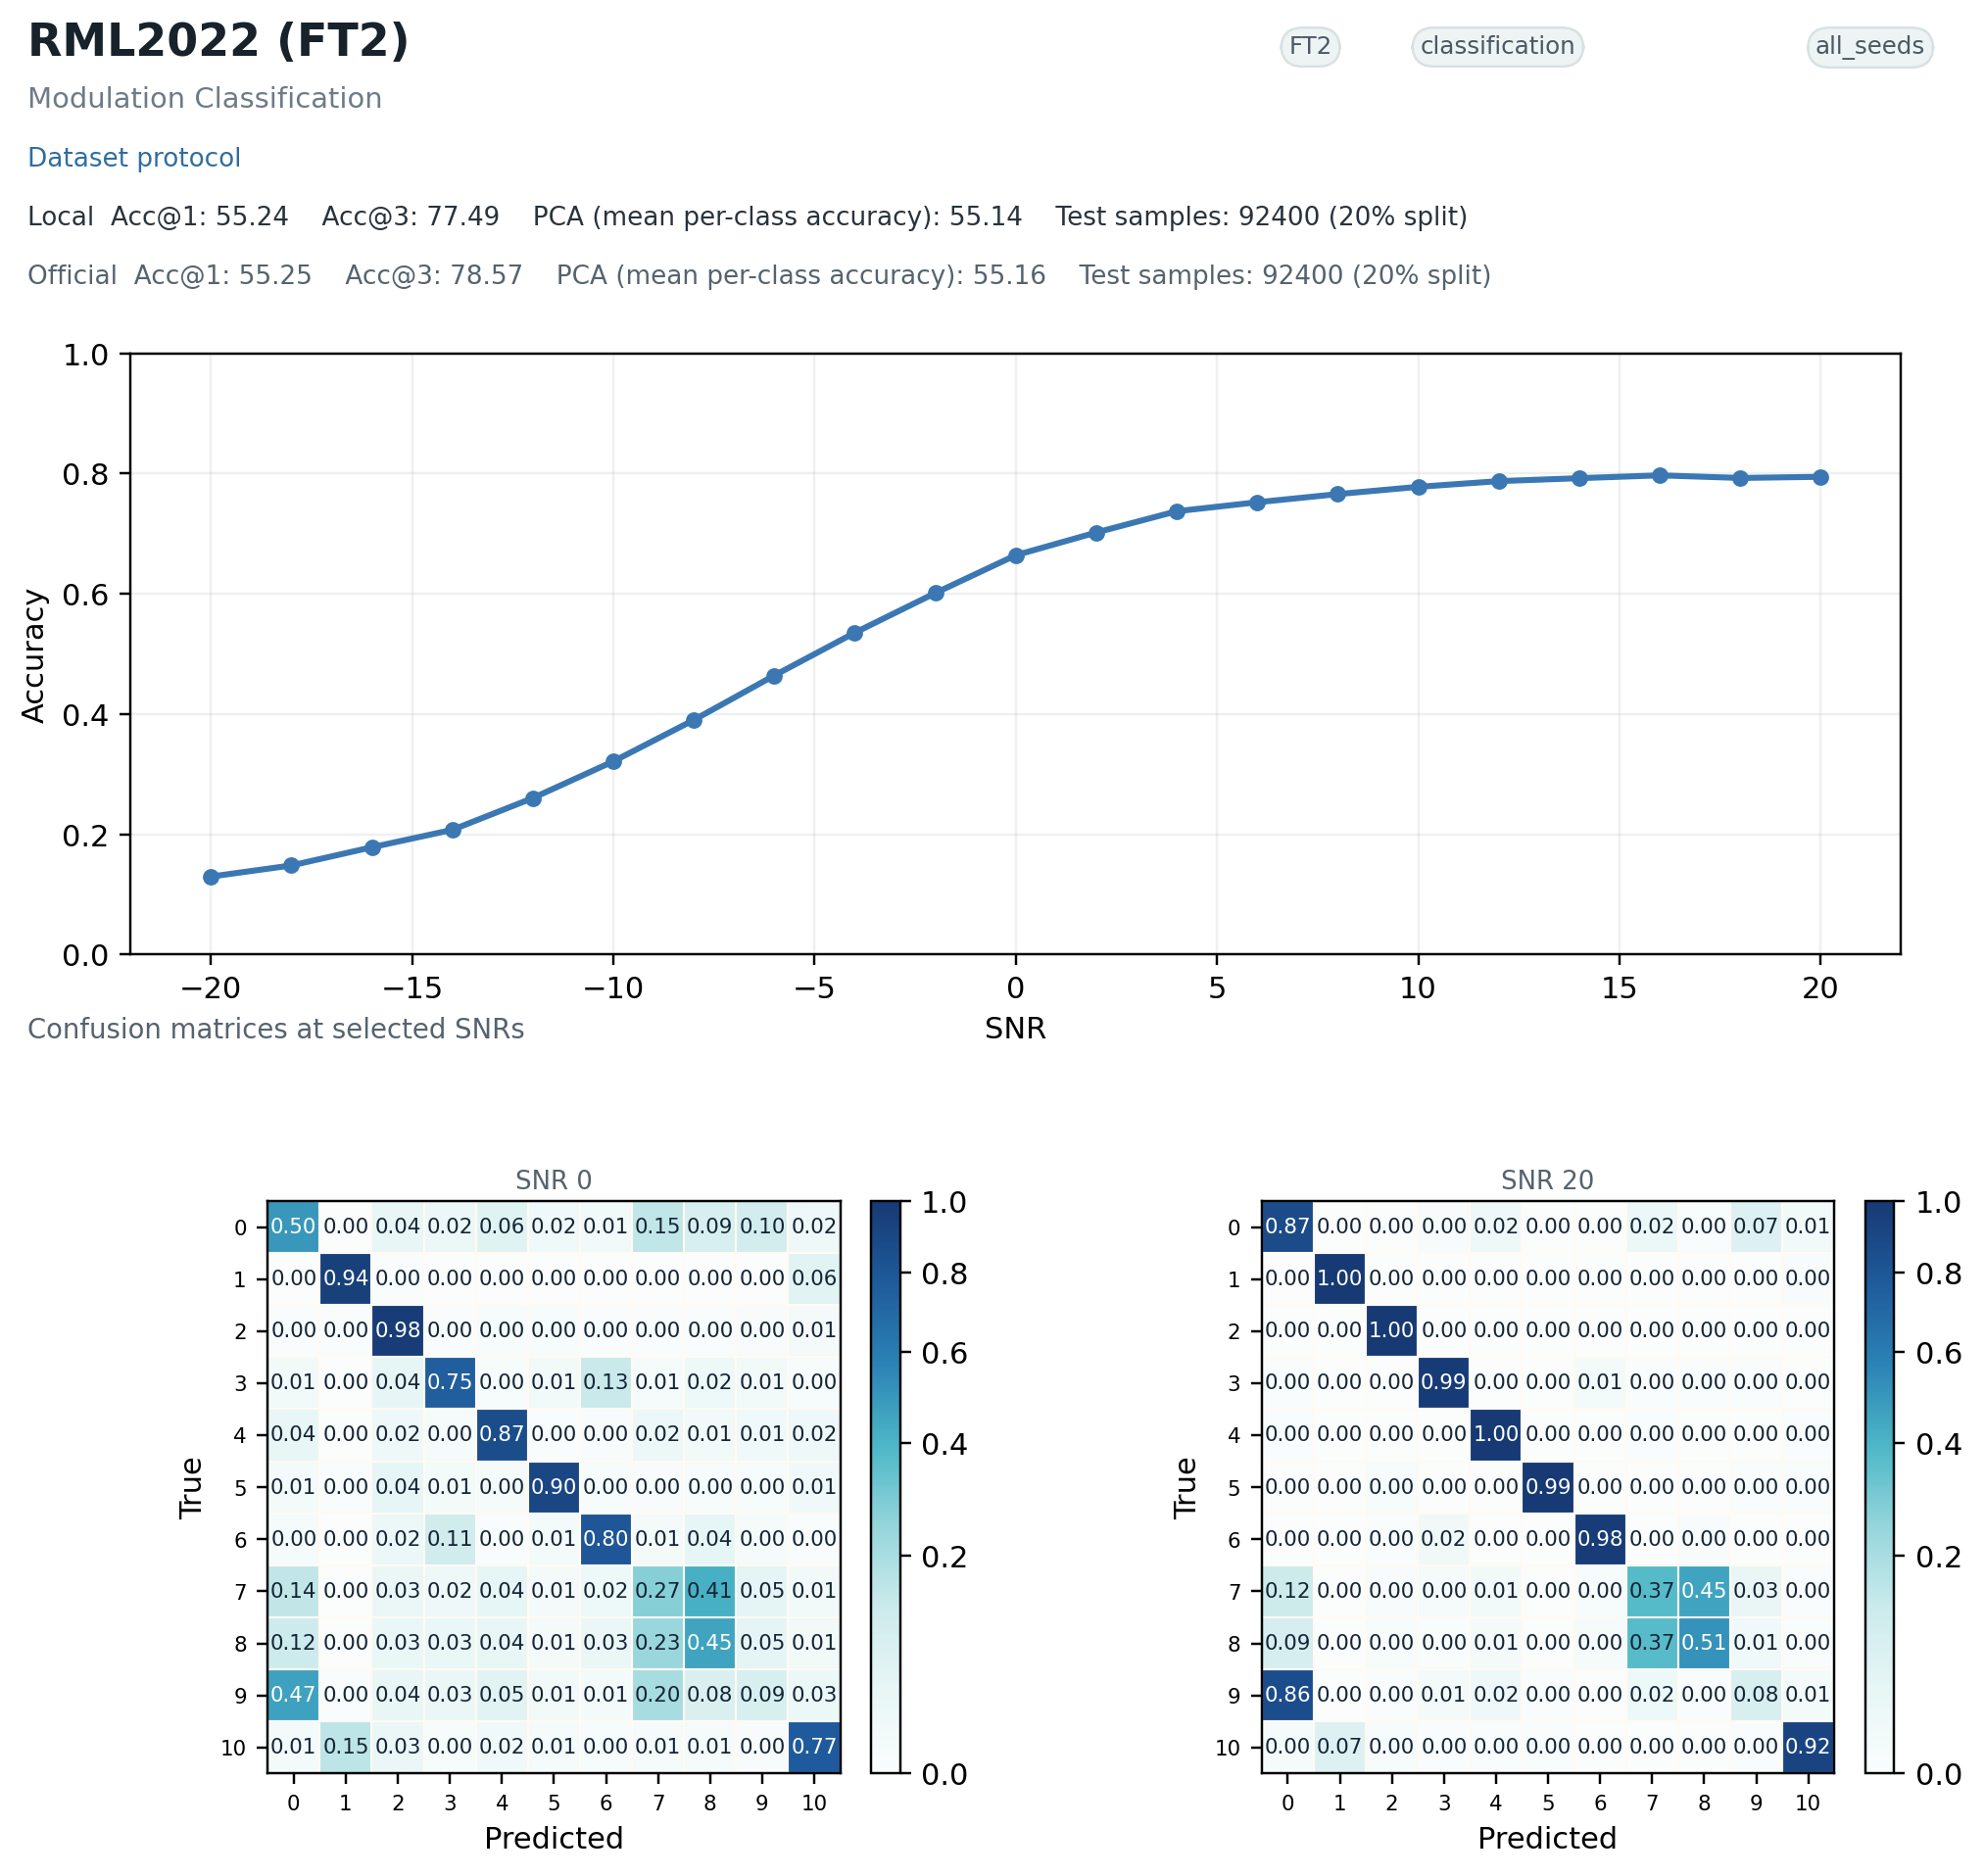
\includegraphics[width=0.75\textwidth]{rml_ft2_overview.png}
    \caption{RML modulation classification overview for FT2, showing per-class performance across 11 modulation types.}
    \label{fig:rml_overview}
\end{figure}

\subsection{Human Activity Sensing: Close, With a Split Caveat}

Sensing results were close to official values (within about 1 percentage point) but showed higher variance across seeds, partly due to the small test set (only 240 samples).

\begin{table}[H]
\centering
\caption{Human activity sensing results (PCA \%, corrected second pass). ``Std'' is the standard deviation across 3 random seeds.}
\label{tab:sensing}
\begin{tabular}{l >{\columncolor{officialbg}}c >{\columncolor{localbg}}c cc}
\toprule
\textbf{Mode} & {\color{officialblue}\textbf{Official}} & {\color{localgreen}\textbf{Local (Mean)}} & \textbf{Std} & \textbf{$\Delta$} \\
\midrule
LP   & 94.42 & 93.89 & 1.99 & $-$0.53 \\
FT2  & 99.31 & 98.47 & 0.86 & $-$0.84 \\
LoRA & 98.47 & 99.31 & 0.71 & $+$0.84 \\
\bottomrule
\end{tabular}
\end{table}

The caveat involves the \textit{data split protocol}---how the data is divided into training and validation sets. The WavesFM preprocessing code merges the original dataset's \code{train} and \code{test} directories into one pool and applies a new random 80/20 split. The exact split indices used for the published numbers are not available. The second pass used a deterministic stratified split, which comes close but cannot be guaranteed to match exactly. With only 240 test samples, even small split differences can shift PCA by 1--2 percentage points.

\begin{figure}[H]
    \centering
    \begin{subfigure}[b]{0.48\textwidth}
        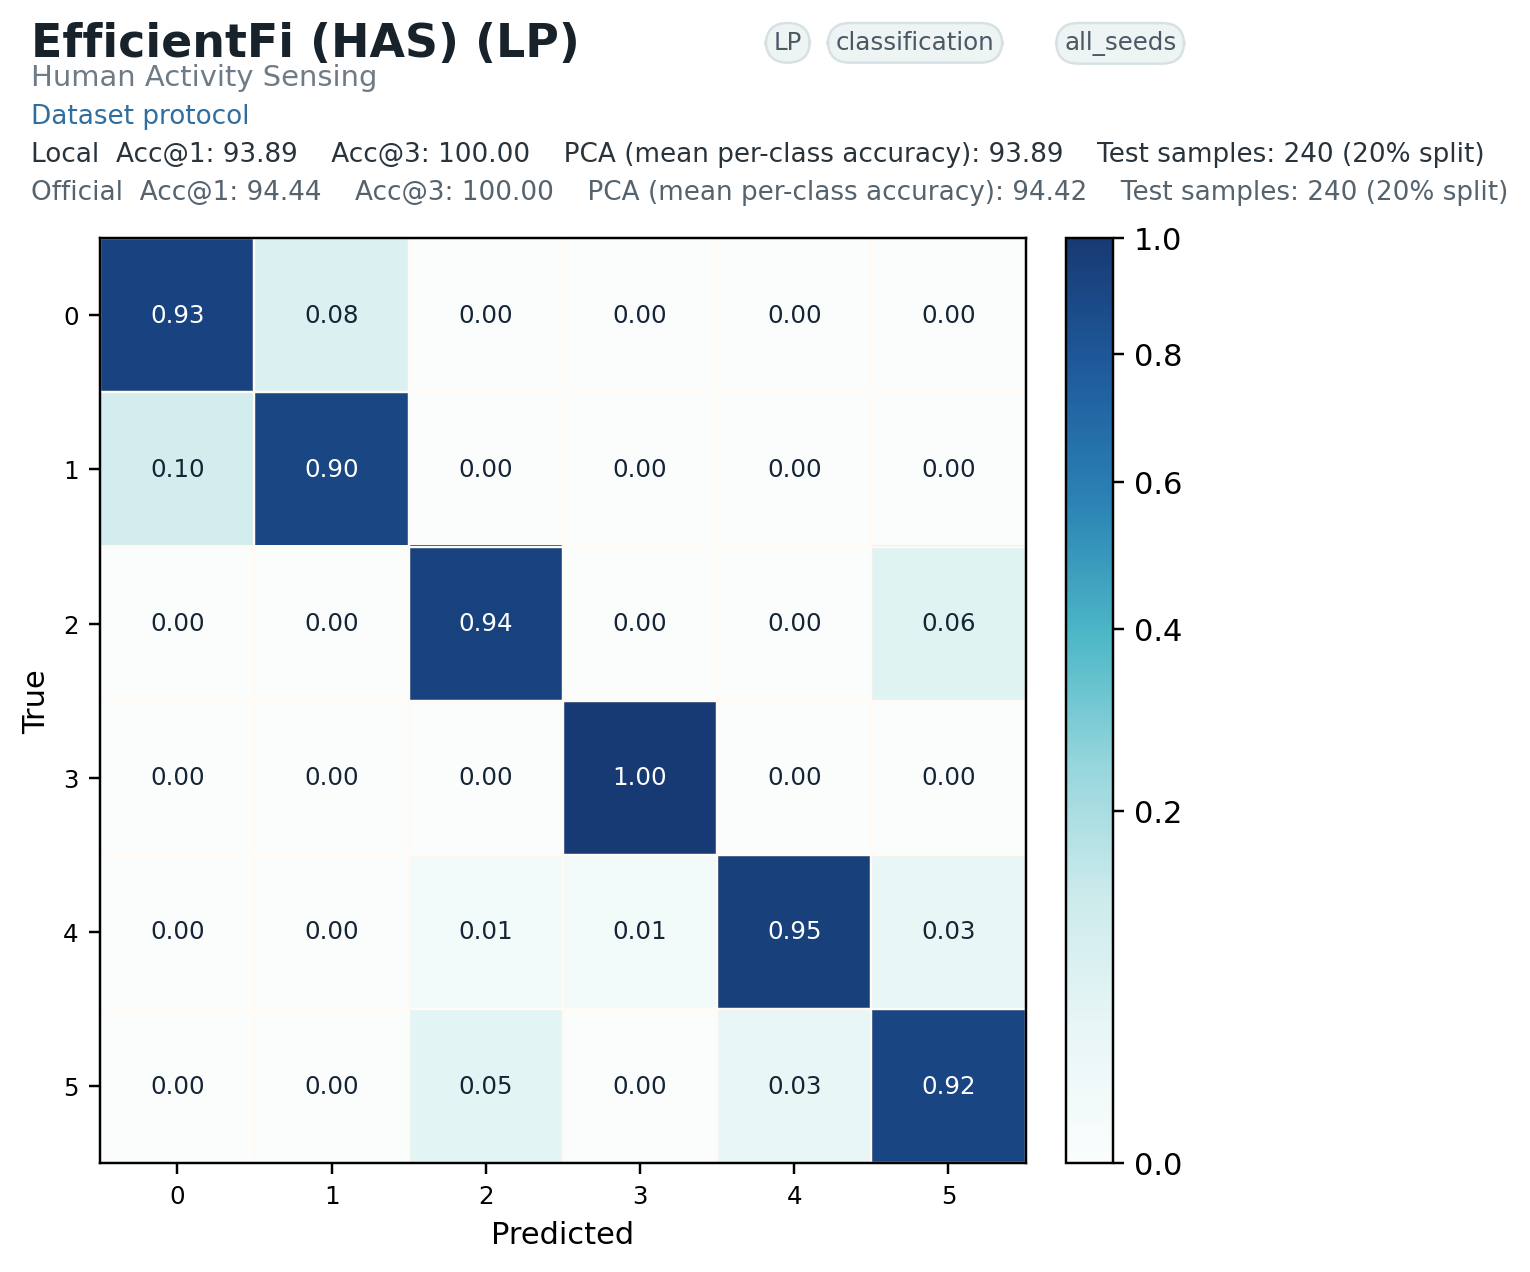
\includegraphics[width=\textwidth]{sensing_lp_cm.png}
        \caption{LP}
    \end{subfigure}
    \begin{subfigure}[b]{0.48\textwidth}
        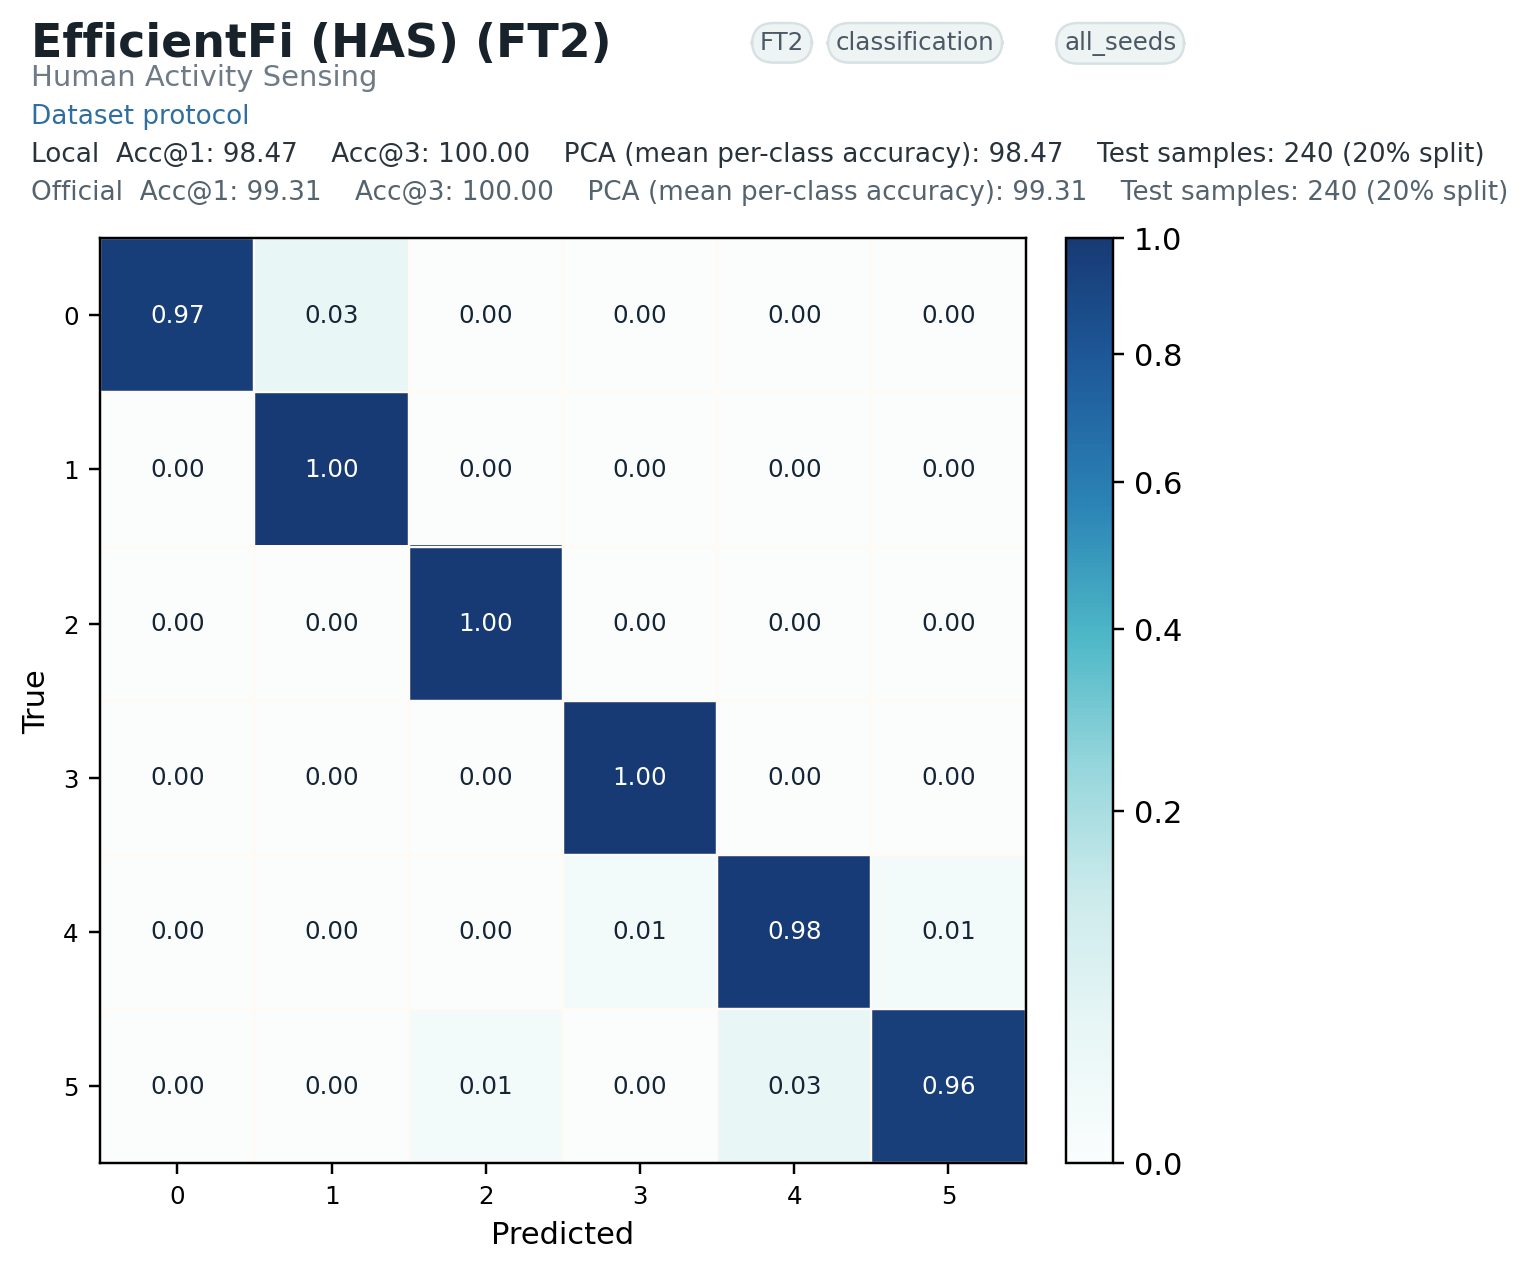
\includegraphics[width=\textwidth]{sensing_ft2_cm.png}
        \caption{FT2}
    \end{subfigure}
    \begin{subfigure}[b]{0.48\textwidth}
        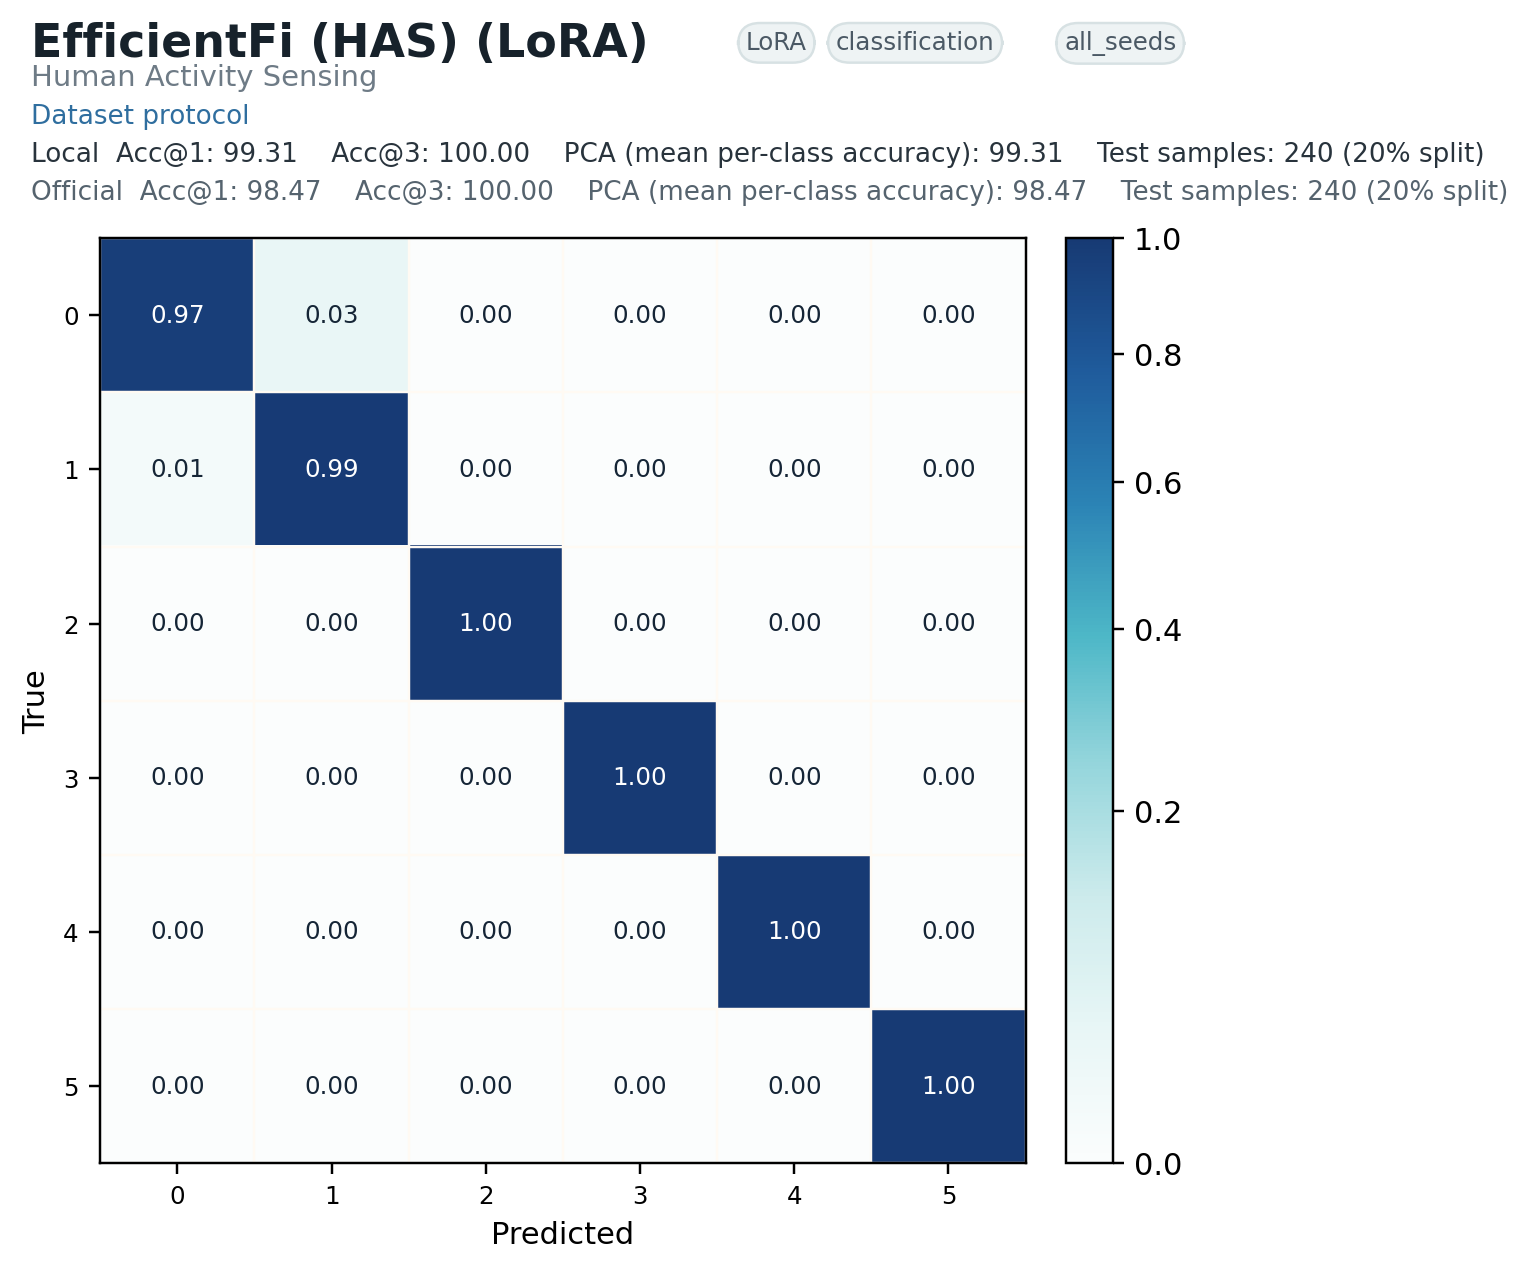
\includegraphics[width=\textwidth]{sensing_lora_cm.png}
        \caption{LoRA}
    \end{subfigure}
    \caption{Confusion matrices for human activity sensing (6 activity classes).}
    \label{fig:sensing_cm}
\end{figure}


\subsection{DeepMIMO Beam Prediction: Not Reproduced}
\label{subsec:beam}

This is the most significant negative finding. Beam prediction showed a persistent gap of 9--11 percentage points below official results, and the gap was highly consistent across seeds (standard deviation $\leq$ 0.64, far smaller than the gap itself).

\begin{table}[H]
\centering
\caption{DeepMIMO beam prediction results (PCA \%, corrected second pass). The large gaps ($\Delta$) highlighted in {\color{gapred}red} show the persistent discrepancy.}
\label{tab:beam}
\begin{tabular}{l >{\columncolor{officialbg}}c >{\columncolor{localbg}}c cc}
\toprule
\textbf{Mode} & {\color{officialblue}\textbf{Official}} & {\color{localgreen}\textbf{Local (Mean)}} & \textbf{Std} & \textbf{$\Delta$} \\
\midrule
LP   & 67.67 & {\color{gapred}56.37} & 0.64 & {\color{gapred}$-$11.30} \\
FT2  & 78.38 & {\color{gapred}69.44} & 0.15 & {\color{gapred}$-$8.94} \\
LoRA & 77.38 & {\color{gapred}67.84} & 0.42 & {\color{gapred}$-$9.54} \\
\bottomrule
\end{tabular}
\end{table}

\noindent\textit{Note: Confusion matrix plots for the 64-class beam prediction task are omitted because a $64 \times 64$ grid is too dense to read at any practical print size. The numerical comparison in Table~\ref{tab:beam} above clearly shows the gap.}

\subsubsection{Three Attempts to Close the Gap}

\paragraph{Attempt 1: First pass (discarded).} Used a pickle-sourced cache that turned out to have only 63 usable beam classes instead of 64. A bug in the beam angle sweep duplicated one endpoint, leaving the top class unreachable. These results were invalidated.

\paragraph{Attempt 2: Corrected second pass.} Rebuilt the cache from official DeepMIMO scenario folders with the beam sweep bug fixed. Verified all 64 beam classes were present. The gap shrank slightly but remained at 9--11 percentage points.

\paragraph{Attempt 3: Alternative data source hypothesis.} Tested whether the official numbers might have been produced from a different data source---the public LWM beam-challenge files (622 labeled samples). Results were near-random (PCA $\approx$ 1.7\%), conclusively ruling out this hypothesis.

\begin{table}[H]
\centering
\caption{LWM beam-challenge hypothesis test (PCA \%). {\color{officialblue}Official beam reference} vs.\ {\color{localgreen}LWM result}. Near-random performance rules out this data source.}
\label{tab:lwm}
\begin{tabular}{l >{\columncolor{officialbg}}c >{\columncolor{localbg}}c cc}
\toprule
\textbf{Mode} & {\color{officialblue}\textbf{Beam Ref}} & {\color{localgreen}\textbf{LWM Result}} & \textbf{Std} & \textbf{$\Delta$} \\
\midrule
LP   & 67.67 & {\color{gapred}1.88} & 0.37 & {\color{gapred}$-$65.79} \\
FT2  & 78.38 & {\color{gapred}1.68} & 0.07 & {\color{gapred}$-$76.70} \\
LoRA & 77.38 & {\color{gapred}1.69} & 0.18 & {\color{gapred}$-$75.69} \\
\bottomrule
\end{tabular}
\end{table}

\noindent The near-random PCA values (around 1.7\% on a 64-class problem, where random chance is $100/64 \approx 1.6\%$) indicate the model learned nothing useful from this data source.

\subsubsection{Why This Gap Exists}

The gap is \textit{not} caused by:
\begin{itemize}
    \item \textbf{Random seed variation}---the standard deviation across seeds is $\leq$ 0.64\%, while the gap is $\geq$ 8.94\%.
    \item \textbf{The 63-class bug}---this was fixed before the second pass.
    \item \textbf{A different data source}---the LWM hypothesis was conclusively rejected.
    \item \textbf{A broken pipeline}---the same code and preprocessor reproduced DeepMIMO LoS/NLoS within 0.10 pp.
\end{itemize}

The most likely explanation is a \textit{benchmark protocol mismatch}: the exact preprocessed data cache, the label-to-beam mapping, or the train/test split indices used for the official evaluation are not recoverable from the publicly available artifacts. The locally reconstructed cache contains 14,840 samples of shape $(2, 32, 32)$, but without access to the exact official cache or split, the gap cannot be closed. This is a \textbf{public artifact availability issue}, not a bug in the reproduction pipeline.


% ============================================================
%  8  Discussion
% ============================================================
\section{Discussion}
\label{sec:discussion}

\subsection{Implications for the WavesFM Claims}

The reproduction results largely support WavesFM's central claim---that a single multimodal ViT backbone can transfer to diverse wireless tasks. Eight tasks reproduced closely, spanning IQ-based tasks (fingerprinting, modulation recognition, interference detection, UWB localization), vision-based tasks (positioning, LoS/NLoS, RADCOM classification), and both classification and regression.

The linear probing results are particularly telling. Under LP, the encoder is completely frozen---no adaptation occurs. If the pretrained features were only useful for one narrow problem, LP would fail on everything else. Instead, LP performed respectably across the board, indicating that self-supervised pretraining on wireless data does produce broadly transferable representations.

\subsection{The Beam Prediction Problem}

The beam prediction failure is notable from a reproducibility standpoint. It is not a case of broken code---the same codebase reproduced 8 other tasks and even reproduced the other DeepMIMO task (LoS/NLoS) from the same dataset. The issue is narrowly scoped to the beam prediction label and split protocol.

This pattern---where the code and model are functional but one specific benchmark cannot be reconstructed from public artifacts---is a recognized challenge in machine learning reproducibility. It underlines why publishing code alone is insufficient for full reproducibility; exact preprocessed data caches and split indices are also needed.

\subsection{The Role of Dataset Size}

A clear pattern emerged: tasks with large test sets (RFP: 208,894 samples; RML: 92,400; RADCOM: 113,400) reproduced with high precision, while tasks with small test sets (sensing: 240; interference: 500) showed more variability. This is statistically expected---smaller samples produce noisier metric estimates---but it has practical implications. Publishing exact split indices becomes especially important for small-dataset tasks, where minor split differences can shift results meaningfully.

\subsection{Practical Considerations}

For researchers considering WavesFM as a starting point:
\begin{itemize}
    \item The pretrained checkpoint transfers effectively across diverse wireless tasks.
    \item The code needs minor fixes before first use (two bug fixes, plus hardware adaptations if not using CUDA).
    \item Most benchmark numbers are reproducible from the public artifacts.
    \item The beam prediction gap is specific to the DeepMIMO beam task and does not undermine the broader model.
    \item The full benchmark suite (90+ runs) requires a capable GPU and some form of automated job management.
\end{itemize}

% ============================================================
%  9  Conclusion
% ============================================================
\section{Conclusion}
\label{sec:conclusion}

This reproducibility study of WavesFM yielded the following findings:

\paragraph{Successfully reproduced (8 tasks).} RF fingerprinting, modulation classification, 5G NR positioning, UWB indoor and industrial localization, RADCOM signal classification, ICARUS interference classification, and DeepMIMO LoS/NLoS all reproduced within a fraction of a percentage point. These span both modality families and both task types, confirming that the WavesFM pretrained backbone transfers across diverse wireless problems.

\paragraph{Closely reproduced with caveat (1 task).} Human activity sensing reproduced within approximately 1 percentage point, but the exact data split used for the official numbers is not published, creating an inherent verification gap on this small dataset.

\paragraph{Not reproduced (1 task).} DeepMIMO beam prediction showed a persistent 9--11 percentage point gap across three experimental attempts. The most likely cause is an unpublished benchmark artifact (data cache or split indices).

\paragraph{Blocked (1 task).} RF signal classification could not be attempted because the publicly available CommRad data format does not match what the preprocessing code expects.

\paragraph{Overall assessment.} WavesFM is a genuine contribution to wireless AI. The multimodal foundation model concept is well-motivated, the architecture functions as described, and the majority of the benchmark reproduces closely. Three additions would achieve full reproducibility: (1)~the exact preprocessed HDF5 caches used for official evaluation, (2)~the exact train/validation split indices for all tasks, and (3)~a tested end-to-end reproduction script that runs without requiring bug fixes.

% ============================================================
%  References
% ============================================================
\begin{thebibliography}{10}

\bibitem{wavesfm_paper}
A.~Aboulfotouh and H.~Abou-Zeid, ``Multimodal wireless foundation models,'' \textit{arXiv:2511.15162v2}, Feb.\ 2026.\\
\url{https://arxiv.org/abs/2511.15162}

\bibitem{wavesfm_original}
A.~Aboulfotouh, E.~Mohammed, and H.~Abou-Zeid, ``6G WavesFM: A foundation model for sensing, communication, and localization,'' \textit{IEEE Open J.\ Commun.\ Soc.}, vol.~6, 2025.\\
\url{https://arxiv.org/abs/2504.14100}

\bibitem{wavesfm_home}
WavesFM project homepage --- code, pretrained weights, benchmark results, dataset documentation, and reproduction instructions.\\
\url{https://wavesfm.waveslab.ai/}

\bibitem{wavesfm_reproduce}
WavesFM reproduction instructions.\\
\url{https://wavesfm.waveslab.ai/docs/reproduce/}

\bibitem{wavesfm_detailed_eval}
WavesFM detailed evaluation results (official baseline numbers used in this study).\\
\url{https://wavesfm.waveslab.ai/detailed-eval/}

\bibitem{zahid2024commrad}
M.~Zahid, ``CommRad RF: A dataset of communication radio signals for detection, identification and classification,'' Zenodo, 2024.\\
\url{https://zenodo.org/records/14192970}

\bibitem{dosovitskiy2021vit}
A.~Dosovitskiy \textit{et al.}, ``An image is worth 16x16 words: Transformers for image recognition at scale,'' in \textit{Proc.\ ICLR}, 2021.\\
\url{https://arxiv.org/abs/2010.11929}

\bibitem{he2022mae}
K.~He \textit{et al.}, ``Masked autoencoders are scalable vision learners,'' in \textit{Proc.\ IEEE/CVF CVPR}, 2022.\\
\url{https://arxiv.org/abs/2111.06377}

\end{thebibliography}


% ============================================================
%  Appendix
% ============================================================
\newpage
\appendix

\section{Per-Seed Variability}
\label{app:seeds}

Table~\ref{tab:seed_std} shows how much results varied across the three random seeds (0, 1, 2). Low standard deviation indicates stable, reliable results; high standard deviation suggests sensitivity to random factors.

\begin{table}[H]
\centering
\caption{Standard deviation across 3 seeds for all task/mode combinations.}
\label{tab:seed_std}
\small
\begin{tabular}{lccc}
\toprule
\textbf{Task} & \textbf{LP Std} & \textbf{FT2 Std} & \textbf{LoRA Std} \\
\midrule
\code{rfp} (PCA \%)            & 0.016 & 0.015 & 0.012 \\
\code{rml} (PCA \%)            & 0.096 & 0.166 & 0.084 \\
\code{radcom} (PCA \%)         & 0.052 & 0.052 & 0.319 \\
\code{interf} (PCA \%)         & 1.225 & 1.381 & 0.624 \\
\code{deepmimo-los} (PCA \%)   & 0.610 & 0.390 & 0.393 \\
\code{sensing} (PCA \%)        & 1.993 & 0.856 & 0.708 \\
\code{deepmimo-beam} (PCA \%)  & 0.640 & 0.147 & 0.418 \\
\code{pos} (meters)            & 0.036 & 0.084 & 0.068 \\
\code{uwb-indoor} (meters)     & 0.019 & 0.006 & 0.016 \\
\code{uwb-industrial} (meters) & 0.010 & 0.010 & 0.007 \\
\bottomrule
\end{tabular}
\end{table}

Tasks with large test sets (\code{rfp}, \code{rml}, \code{radcom}) show very low variance. Tasks with small test sets (\code{sensing}: 240 samples, \code{interf}: 500 samples) show higher variance, as expected.

\section{Complete Code Change Log}
\label{app:code_changes}

All modifications to the released \code{wavesfm/} codebase, by file:

\begin{enumerate}
    \item \code{run\_finetune\_all.py}: Removed broken import; changed default beams 16$\to$64; added \code{sensing} to stratified split set.
    \item \code{main\_finetune.py}: Device auto-selection; AMP restricted to CUDA; default beams 16$\to$64; atomic checkpoint writes; RNG state save/restore; safe DataLoader tuning.
    \item \code{utils.py}: NumPy seeding; fsynced JSONL logging; worker-seeding helpers.
    \item \code{preprocess\_uwb\_loc.py}: Removed non-existent \code{args.root} reference (bug fix).
    \item \code{preprocess\_deepmimo.py}: Half-open beam sweep fix; pickle input support; cache audit attributes; full-length class weights.
    \item \code{preprocess\_radcom.py}: Single-pass statistics accumulation (same output).
    \item \code{preprocess\_csi\_sensing.py}: Source-split provenance tracking; cache version v1$\to$v2.
    \item \code{preprocess\_lwm\_beam\_challenge.py}: New preprocessor for hypothesis test.
    \item \code{data.py}: Beam head sized from codebook; added \code{lwm-beam-challenge} task.
    \item \code{dataset\_classes/deepmimo.py}: Beam cache validation; malformed-cache warnings.
    \item \code{requirements.txt}: Added \code{matplotlib==3.10.7}.
\end{enumerate}

\section{Experimental Session Details}
\label{app:sessions}

\begin{description}
    \item[First full run] \code{20260403\_004122-ngwn06}\\
    10 tasks $\times$ 3 modes $\times$ 3 seeds = 90 runs. Host: \code{ngwn06} (RTX 5090, 24 cores, 62\,GB RAM). All 90 completed. Final results for 7 tasks.

    \item[Corrected second pass] \code{second\_try\_sensing\_deepmimo\_20260415\_005633-ngwn06}\\
    3 tasks $\times$ 3 modes $\times$ 3 seeds = 27 runs. Same host. All 27 completed. Final results for \code{sensing}, \code{deepmimo-los}, and \code{deepmimo-beam}.

    \item[Hypothesis test] \code{third\_try\_lwm\_beam\_challenge\_20260415\_140720-ngwn06}\\
    1 task $\times$ 3 modes $\times$ 3 seeds = 9 runs. Same host. All 9 completed. Diagnostic only---conclusive negative result.
\end{description}

\end{document}
